\documentclass[a4paper,13pt]{report}

% --------------------------------------------------------------------
% Compile instructions:
% - To compile with XeLaTeX (recommended for Times New Roman and Unicode):
%     latexmk -pdfxe thesis.tex
%   or
%     xelatex thesis.tex
%
% - To compile with LuaLaTeX, use:
%     latexmk -pdflua thesis.tex
%
% - To compile with pdfLaTeX (default behaviour):
%     latexmk -pdf thesis.tex
%   (This uses Latin Modern and T5 encoding for Vietnamese.)
% --------------------------------------------------------------------

% Encoding and Vietnamese support
% This file supports both pdfLaTeX and XeLaTeX/LuaLaTeX. The default
% behaviour below keeps the existing pdfLaTeX setup (Latin Modern + T5
% encoding for Vietnamese). If you switch to XeLaTeX/LuaLaTeX, the
% document will use system fonts via `fontspec` (set to Times New Roman).
\usepackage{iftex}
\ifPDFTeX
	% pdfLaTeX: keep older encoding packages and Latin Modern.
	\usepackage[utf8]{inputenc} % keep for pdfLaTeX; not used with XeLaTeX
	\usepackage[T5]{fontenc}    % T5 encoding (Vietnamese) - required for vntex/vietnam
	\usepackage[utf8]{vietnam}  % Vietnamese support (vntex)
	% If you want a Times-like font with pdfLaTeX you can enable the
	% following packages, but note: T5 encoding support and some
	% Vietnamese glyphs may not be complete with these fonts. Test the
	% output before enabling.
	% \usepackage{newtxtext,newtxmath} % Times-like fonts (for pdfLaTeX)
\else
	% XeLaTeX/LuaLaTeX: use fontspec and polyglossia for Unicode & Vietnamese
	% NOTE: If your source uses TeX accent macros (e.g., `\h{a}` or `\'a`)
	% instead of raw Unicode characters, you may need to either (A) keep
	% the `vietnam` package loaded or (B) convert source files to Unicode
	% characters for Vietnamese. Loading both `polyglossia` and `vietnam`
	% may cause conflicts; test carefully.
	\usepackage{fontspec}
	\usepackage{polyglossia}
	% If your source contains TeX accent macros rather than raw Unicode
	% characters (e.g. `\h{a}`), uncomment the following line to load
	% the `vietnam` package which defines such macros. Keep in mind
	% that `vietnam` is designed for T5 encoding and may sometimes
	% overlap with `polyglossia` macros.
	\usepackage[utf8]{vietnam}
	\setmainlanguage{vietnamese}
	% Set Times New Roman as the main font. You can change the name if
	% your OS has a differently named Times family (e.g., "Times").
	\setmainfont{Times New Roman}[
		Ligatures=TeX,
		Script=Latin
	]
	% If you want math fonts to match Times, you can add e.g.:
	% \usepackage{unicode-math}
	% \setmathfont{TeX Gyre Termes Math}
	% Optional: specify sans/mono fonts to better match system defaults
	\setsansfont{Arial}
	\setmonofont{Courier New}
\fi
\usepackage{amsmath, amsfonts, amssymb}
\usepackage{textcomp}

% Note: If you prefer to compile with XeLaTeX or LuaLaTeX (recommended for Unicode):
%  - remove or comment out the `inputenc` and `fontenc` lines above
%  - uncomment the fontspec lines below and set an appropriate system font
%  - compile with: `latexmk -pdfxe thesis.tex` or `latexmk -pdflua thesis.tex`
%
% %%% XeLaTeX / LuaTeX example (uncomment when using XeLaTeX/LuaTeX):
% \usepackage{fontspec}
% \setmainfont{Times New Roman}
% \usepackage{polyglossia}
% \setmainlanguage{vietnamese}

% set font, font size and spacing
% If compiling with pdfLaTeX, keep Latin Modern for T5 coverage. For
% XeLaTeX/LuaLaTeX the fontspec package (above) will set Times.
\ifPDFTeX
	\usepackage{lmodern}
\fi
\usepackage{microtype} % micro-typography
\usepackage{scrextend}
\changefontsizes{13pt}
\renewcommand{\baselinestretch}{1.3}

% Hình ảnh và đồ họa
\usepackage{graphicx}
\usepackage{tikz}
\usetikzlibrary{shapes.geometric, arrows, positioning, arrows.meta, calc, fit}
% PGFPlots: required for axis environment and plotting
\usepackage{pgfplots}
\pgfplotsset{compat=1.18}
% Disable thousand separators by default for axis tick labels (e.g., 1990 shows as 1990, not 1,990)
\pgfplotsset{every axis/.append style={xticklabel style={/pgf/number format/1000 sep={}}}}
\usepackage[justification=centering]{caption}

% Định dạng bảng và caption
\usepackage{booktabs}
\usepackage[font=small]{caption}
\usepackage{makecell}
\usepackage{multirow}

% Điều chỉnh lề và layout trang
\usepackage[left=3cm,right=2cm,top=2.5cm,bottom=3cm]{geometry}

% Hyperlinks và danh mục
\usepackage[unicode]{hyperref}

% Định dạng tiêu đề chương, mục
\usepackage{titlesec} 
\titleformat{\chapter}[display]
{\raggedright\large}
{\MakeUppercase{\chaptertitlename}~\thechapter}
{0pt}
{\vspace{2\baselineskip}\bfseries\huge}
%\titlespacing*{\chapter}{0cm}{-\topskip}{0pt}[0pt]

\titleformat{\chapter}[block]{\normalfont\Large\bfseries}{\thechapter.}{1em}{}
\renewcommand{\contentsname}{\MakeUppercase{MỤC LỤC}} 

% Tùy chỉnh các phần khác
\usepackage{scrextend, enumerate, float, afterpage, sectsty, tocloft, calc, listings}

\usepackage{pdflscape} % Gói giúp xoay trang ngang trong PDF
\usepackage{graphicx}
\usepackage{float} % Để cố định vị trí bảng
\graphicspath{{img/}{img/chapter1/}{img/chapter2/}{img/chapter3/}{img/chapter4/}{img/chapter5/}}
\usepackage{longtable} % Nếu bảng dài
\usepackage{lscape} % Để hỗ trợ xoay trang (tuỳ chọn)

% Gói hỗ trợ thuật toán
\usepackage[linesnumbered,ruled,vlined]{algorithm2e}
\usepackage{optidef}

% Điều chỉnh các thuật toán
\SetAlgorithmName{Thuật toán}{Thuật toán}{Danh sách các Thuật toán}
\SetKwInput{KwIn}{Đầu vào}
\SetKwInput{KwOut}{Đầu ra}

% Định dạng danh mục tài liệu tham khảo
\usepackage[numbers,sort&compress]{natbib}

% Định dạng lại các tiêu đề section và subsection
\sectionfont{\fontsize{15}{15}\selectfont}
\subsectionfont{\fontsize{13}{15}\selectfont}

% Điều chỉnh khoảng cách giữa các đoạn
\usepackage{indentfirst}
\setlength{\parskip}{6pt}
\setlength{\parindent}{1cm}

% Tùy chỉnh chú thích
\usepackage{perpage} 
\MakePerPage{footnote}

% Khoảng cách dòng
\renewcommand{\baselinestretch}{1.3}

% Tùy chỉnh mục lục
\renewcommand{\cftchappresnum}{Chương }
\AtBeginDocument{\addtolength\cftchapnumwidth{\widthof{\bfseries Chương }}}

% Thiết lập tiêu đề và tác giả
\title{Ứng dụng viễn thám và học sâu trong giám sát biến động rừng tỉnh Cà Mau}
\author{Ninh Hải Đăng} 

% Khai báo các thư viện cho mục lục hình ảnh và bảng
\def\l@figure{\@dottedtocline{1}{1em}{2.2em}}
\def\l@table{\@dottedtocline{1}{1em}{2.2em}}

\newcommand{\argmax}{\arg\!\max}

\begin{document}
% Bìa chính và các phần đầu
% Cover Vietnamese 1

% Cover english
\pagenumbering{gobble}
\begin{center}
	\begin{tikzpicture}[overlay,remember picture]
	    \draw [line width=3pt,rounded corners=0pt,
	        ]
	        ($ (current page.north west) + (25mm,-25mm) $)
	        rectangle
	        ($ (current page.south east) + (-15mm,25mm) $);
	    \draw [line width=1pt,rounded corners=0pt]
	        ($ (current page.north west) + (26.5mm,-26.5mm) $)
	        rectangle
	        ($ (current page.south east) + (-16.5mm,26.5mm) $);
	\end{tikzpicture}
	\\[1mm]
	%%12pt
	\textbf{ĐẠI HỌC QUỐC GIA HÀ NỘI\\TRƯỜNG ĐẠI HỌC CÔNG NGHỆ}\\[1cm]
	\includegraphics[width=0.2\linewidth]{img/uet}\\[0.3cm]
	{\fontsize{14pt}{16pt}\selectfont\textbf{Ninh Hải Đăng}}
	\\[2cm]

	{\fontsize{18pt}{22pt}\selectfont\textbf{ỨNG DỤNG VIỄN THÁM VÀ HỌC SÂU TRONG \\ GIÁM SÁT BIẾN ĐỘNG RỪNG TỈNH CÀ MAU}}
	\\[2.6cm]
	{\fontsize{14pt}{16pt}\selectfont\textbf{ĐỒ ÁN TỐT NGHIỆP ĐẠI HỌC HỆ CHÍNH QUY
			\\[2mm]
			Ngành: Công nghệ Hàng không Vũ trụ}}

	\vfill
	{\fontsize{12pt}{14pt}\selectfont\textbf{HÀ NỘI - 2025}}
	\vspace{10mm}
\end{center}

\begin{center}
	\begin{tikzpicture}[overlay,remember picture]
	\draw [line width=3pt,rounded corners=0pt]
	($ (current page.north west) + (25mm,-25mm) $)
	rectangle
	($ (current page.south east) + (-15mm,25mm) $);
	\draw [line width=1pt,rounded corners=0pt]
	($ (current page.north west) + (26.5mm,-26.5mm) $)
	rectangle
	($ (current page.south east) + (-16.5mm,26.5mm) $);
	\end{tikzpicture}
	\\[1mm]
	\textbf{ĐẠI HỌC QUỐC GIA HÀ NỘI\\TRƯỜNG ĐẠI HỌC CÔNG NGHỆ}
	\\[1cm]
	\includegraphics[width=0.2\linewidth]{img/uet}
	\\[0.3cm]
	{\fontsize{14pt}{16pt}\selectfont\textbf{Ninh Hải Đăng}}
	\\[2cm]

	{\fontsize{18pt}{22pt}\selectfont\textbf{ỨNG DỤNG VIỄN THÁM VÀ HỌC SÂU TRONG  GIÁM SÁT BIẾN ĐỘNG RỪNG TỈNH CÀ MAU}}
	\\[1.5cm]
{\fontsize{14pt}{16pt}\selectfont\textbf{ĐỒ ÁN TỐT NGHIỆP ĐẠI HỌC HỆ CHÍNH QUY
		\\[2mm]
	Ngành: Công nghệ Hàng không Vũ trụ}}
\end{center}
\vspace{1mm}
\hspace*{12mm}\textbf{Cán bộ hướng dẫn: TS. Hà Minh Cường}
\\[2.5cm]
\hspace*{51mm}\textbf{ThS. Hoàng Tích Phúc}
\vfill
\begin{center}
		{\fontsize{12pt}{14pt}\selectfont\textbf{HÀ NỘI - 2025}}
	\vspace{4mm}
\end{center}
\newpage\cleardoublepage

% Chuyển sang đánh số trang kiểu La Mã
\pagenumbering{roman} 
\phantomsection
\addcontentsline{toc}{chapter}{TÓM TẮT}
\unnumberedchapter{TÓM TẮT}

{\fontsize{12pt}{14pt}\selectfont
\textbf{Tóm tắt:} Đồ án này nghiên cứu ứng dụng mạng Neural Tích chập (CNN) kết hợp với dữ liệu viễn thám đa nguồn từ vệ tinh Sentinel-1 và Sentinel-2 để phát hiện và phân loại biến động rừng tại tỉnh Cà Mau — khu vực rừng ngập mặn quan trọng bậc nhất tại Việt Nam. Nghiên cứu sử dụng 27 đặc trưng bao gồm các kênh phổ, chỉ số thực vật (NDVI, NBR, NDMI) và dữ liệu SAR từ hai thời kỳ (01/2024 và 02/2025) với độ phân giải 10m.

Kiến trúc CNN nhẹ với khoảng 36,000 tham số được thiết kế, sử dụng patches 3×3 để khai thác ngữ cảnh không gian, áp dụng các kỹ thuật regularization (Batch Normalization, Dropout, Weight Decay) để tránh overfitting trên bộ dữ liệu thực địa gồm 2,630 điểm với 4 lớp phân loại: Rừng ổn định, Mất rừng, Phi rừng và Phục hồi rừng. Quy trình đánh giá triển khai với stratified random split kết hợp 5-Fold Cross Validation, đảm bảo phân bố cân bằng các lớp và giữ lại 20\% dữ liệu làm tập test cố định.

Kết quả cho thấy mô hình đạt độ chính xác 98.86\% trên tập test với ROC-AUC 99.98\%, Cross Validation cho kết quả trung bình 98.15\% ± 0.28\% chứng tỏ mô hình ổn định và có khả năng tổng quát hóa tốt. Ứng dụng thực tế phân loại toàn vùng quy hoạch lâm nghiệp Cà Mau với diện tích 170,179 ha, phát hiện 7,282 ha mất rừng (4.48\%) và 4,941 ha phục hồi rừng (3.04\%) trong giai đoạn nghiên cứu, đóng góp phương pháp hiệu quả cho công tác giám sát tài nguyên rừng.

\textbf{\textit{Từ khóa:}} CNN, viễn thám, biến động rừng, Cà Mau.
}
\newpage\cleardoublepage
\phantomsection
\addcontentsline{toc}{chapter}{LỜI CAM ĐOAN}
\unnumberedchapter{LỜI CAM ĐOAN}

Tôi tên là Ninh Hải Đăng, sinh viên lớp QH-2021-I/CQ-S-AE, Viện Công nghệ Hàng không Vũ trụ, Trường Đại học Công nghệ – Đại học Quốc gia Hà Nội. Tôi xin cam đoan rằng Đồ án tốt nghiệp với đề tài ``Ứng dụng viễn thám và học sâu trong giám sát biến động rừng tỉnh Cà Mau'' là kết quả nghiên cứu khoa học do chính tôi thực hiện dưới sự hướng dẫn của TS. Hà Minh Cường và ThS. Hoàng Tích Phúc.

Mọi sự hỗ trợ, hướng dẫn trong quá trình thực hiện đều đã được ghi nhận và cảm ơn; các thông tin, số liệu, tài liệu tham khảo trong đồ án đều được trích dẫn đầy đủ và được phép sử dụng. Tôi xin đảm bảo rằng tất cả dữ liệu nghiên cứu và kết quả trình bày trong đồ án là trung thực và chính xác. Nếu phát hiện bất kỳ sai sót nào, tôi xin hoàn toàn chịu trách nhiệm trước cơ quan nhà trường và các cơ quan liên quan.

\begin{flushright}
    \makebox[5cm][c]{Sinh viên} \\
    \vspace{2cm}
    \makebox[5cm][c]{Ninh Hải Đăng}
\end{flushright}
\newpage\cleardoublepage
\phantomsection
\addcontentsline{toc}{chapter}{LỜI CẢM ƠN}
\unnumberedchapter{LỜI CẢM ƠN}

Trước tiên, em xin chân thành cảm ơn Công ty TNHH Tư vấn và Phát triển Đồng Xanh đã tạo điều kiện cho em thực hiện đề tài thực tập tốt nghiệp này. Môi trường làm việc chuyên nghiệp và sự hỗ trợ nhiệt tình từ công ty đã giúp em có cơ hội áp dụng kiến thức đã học vào thực tiễn.

Em xin gửi lời cảm ơn sâu sắc đến TS. Hoàng Việt Anh - cán bộ hướng dẫn tại công ty, người đã dành thời gian hướng dẫn, giải đáp các thắc mắc và định hướng cho em trong suốt quá trình thực tập.

Em xin chân thành cảm ơn TS. Nguyễn Văn Thương - giảng viên phụ trách bộ môn, cùng TS. Hà Minh Cường và ThS. Hoàng Tích Phúc - các thầy giảng viên hướng dẫn tại Viện Công nghệ Hàng không Vũ trụ, đã tận tình chỉ bảo, theo dõi và hỗ trợ em trong suốt quá trình thực hiện đề tài. Sự hướng dẫn tận tâm của các thầy đã giúp em nâng cao kiến thức chuyên môn và hoàn thiện kỹ năng nghiên cứu khoa học.

Cuối cùng, em xin cảm ơn gia đình, bạn bè và đồng nghiệp đã luôn động viên, chia sẻ và tạo điều kiện tốt nhất để em hoàn thành báo cáo thực tập này.

Do thời gian và kinh nghiệm còn hạn chế, báo cáo không tránh khỏi những thiếu sót. Em rất mong nhận được sự góp ý của quý thầy cô và các bạn để báo cáo được hoàn thiện hơn.

Em xin chân thành cảm ơn!

\vspace{1cm}

\begin{flushright}
\textit{Hà Nội, tháng 12 năm 2025}\\
\textit{Sinh viên}\\[1.5cm]
\textbf{Ninh Hải Đăng}
\end{flushright}
\newpage\cleardoublepage

% Mục lục, danh sách hình ảnh, bảng, thuật toán
\addcontentsline{toc}{chapter}{Mục lục}
\tableofcontents\newpage\cleardoublepage

\addcontentsline{toc}{chapter}{\listfigurename}
\listoffigures\cleardoublepage

\addcontentsline{toc}{chapter}{\listtablename}
\listoftables\cleardoublepage

% Thuật ngữ
\phantomsection
\addcontentsline{toc}{chapter}{DANH MỤC THUẬT NGỮ VÀ TỪ VIẾT TẮT}
\unnumberedchapter{DANH MỤC THUẬT NGỮ VÀ TỪ VIẾT TẮT}

\begin{longtable}{p{5cm} c p{6cm}}
\centering\textbf{Từ} & \textbf{Viết tắt} & \centering\arraybackslash\textbf{Dịch - Nghĩa} \\[0.3cm]
Ablation Study & - & Nghiên cứu loại trừ (phân tích ảnh hưởng từng thành phần) \\
Accuracy & - & Độ chính xác tổng thể (tỷ lệ dự đoán đúng trên tổng số mẫu) \\
Activation Function & - & Hàm kích hoạt (hàm phi tuyến trong mạng nơ-ron) \\
AdamW & - & Thuật toán tối ưu Adam với phân rã trọng số tách rời \\
Artificial Intelligence & AI & Trí tuệ nhân tạo \\
Backscatter & - & Tán xạ ngược (năng lượng ra-đa phản hồi về cảm biến) \\
Batch Normalization & BN & Chuẩn hóa theo lô (chuẩn hóa đầu vào mỗi lớp theo mini-batch) \\
Bi-temporal & - & Hai thời điểm (phân tích so sánh hai thời kỳ) \\
C-band & - & Băng tần C (bước sóng ra-đa 4-8 GHz, xuyên qua mây) \\
Classification & - & Phân loại (gán nhãn cho đối tượng) \\
Compute Unified Device Architecture & CUDA & Nền tảng tính toán song song của NVIDIA trên GPU \\
Confusion Matrix & - & Ma trận nhầm lẫn (bảng so sánh dự đoán và thực tế) \\
Convolutional Neural Network & CNN & Mạng nơ-ron tích chập \\
Cross Validation & CV & Kiểm định chéo (đánh giá mô hình trên nhiều phần dữ liệu) \\
CrossEntropyLoss & - & Hàm mất mát entropy chéo (đo độ sai khác phân phối xác suất) \\
Deep Learning & DL & Học sâu (học máy với nhiều lớp ẩn) \\
Deforestation & - & Mất rừng (chuyển đổi từ rừng sang phi rừng) \\
Dropout & - & Loại bỏ ngẫu nhiên (tắt ngẫu nhiên một số nơ-ron khi huấn luyện) \\
Early Stopping & - & Dừng sớm (ngừng huấn luyện khi validation loss không giảm) \\
European Space Agency & ESA & Cơ quan Vũ trụ Châu Âu \\
European Union & EU & Liên minh Châu Âu \\
F1-Score & - & Điểm F1 (trung bình điều hòa của độ chuẩn xác và độ phủ) \\
False Negative & FN & Âm tính giả (dự đoán âm nhưng thực tế dương) \\
False Positive & FP & Dương tính giả (dự đoán dương nhưng thực tế âm) \\
False Positive Rate & FPR & Tỷ lệ dương tính giả \\
Feature & - & Đặc trưng (thuộc tính đầu vào của mô hình) \\
Feature Extraction & - & Trích xuất đặc trưng (rút trích thông tin từ dữ liệu thô) \\
Feature Map & - & Bản đồ đặc trưng (đầu ra của lớp tích chập) \\
Kernel & - & Bộ lọc/Nhân tích chập (ma trận trọng số trượt qua ảnh) \\
Fold & - & Phần gập (một phần dữ liệu trong Cross Validation) \\
Food and Agriculture Organization & FAO & Tổ chức Lương thực và Nông nghiệp Liên Hợp Quốc \\
Forest Change Detection & - & Phát hiện biến động rừng \\
Fully Connected Layer & FC & Lớp kết nối đầy đủ (mỗi nơ-ron kết nối với tất cả nơ-ron lớp trước) \\
Geographic Information System & GIS & Hệ thống thông tin địa lý \\
Global Average Pooling & GAP & Gộp trung bình toàn cục (lấy trung bình toàn bộ bản đồ đặc trưng) \\
Global Forest Watch & GFW & Giám sát rừng toàn cầu \\
Graphics Processing Unit & GPU & Bộ xử lý đồ họa (phần cứng tính toán song song) \\
Ground Truth & - & Dữ liệu mẫu (nhãn thực tế dùng để huấn luyện và đánh giá mô hình, thường thu thập từ khảo sát thực địa hoặc giải đoán ảnh) \\
Hyperparameter & - & Siêu tham số (tham số cấu hình trước khi huấn luyện) \\
Interferometric Wide & IW & Chế độ giao thoa rộng (chế độ chụp chính của Sentinel-1) \\
Intergovernmental Panel on Climate Change & IPCC & Ủy ban Liên chính phủ về Biến đổi Khí hậu \\
Learning Rate & LR & Tốc độ học (bước cập nhật trọng số mỗi lần lặp) \\
Lightweight & - & Kiến trúc nhẹ (mô hình có ít tham số, tính toán nhanh) \\
Logits & - & Giá trị logit (đầu ra thô của mạng trước khi áp dụng softmax) \\
Machine Learning & ML & Học máy \\
Mangrove Forest & - & Rừng ngập mặn \\
Multi-Layer Perceptron & MLP & Perceptron đa lớp (mạng nơ-ron nhiều lớp kết nối đầy đủ) \\
Multispectral & - & Đa phổ (ảnh chụp ở nhiều dải bước sóng) \\
Near-Infrared & NIR & Cận hồng ngoại (bước sóng 0.7--1.4 $\mu$m) \\
Non-forest & - & Phi rừng (vùng không có rừng che phủ) \\
Normalized Burn Ratio & NBR & Chỉ số cháy chuẩn hóa (phát hiện vùng cháy rừng) \\
Normalized Difference Moisture Index & NDMI & Chỉ số độ ẩm chuẩn hóa (đánh giá độ ẩm thực vật) \\
Normalized Difference Vegetation Index & NDVI & Chỉ số thực vật chuẩn hóa (đánh giá mức độ xanh tươi) \\
Optical & - & Quang học (ảnh vệ tinh dùng ánh sáng khả kiến và hồng ngoại) \\
Overfitting & - & Quá khớp (mô hình học thuộc dữ liệu huấn luyện, kém tổng quát) \\
Padding & - & Đệm viền (thêm pixel xung quanh ảnh khi tích chập) \\
Parameter & - & Tham số (trọng số học được trong quá trình huấn luyện) \\
Patch & - & Mảnh ảnh (vùng ảnh nhỏ trích xuất từ ảnh gốc) \\
Pixel & - & Điểm ảnh (đơn vị nhỏ nhất của ảnh số) \\
Polarization & - & Phân cực (hướng dao động của sóng ra-đa: VV, VH) \\
Pooling & - & Gộp (giảm kích thước không gian của feature map) \\
Precision & - & Độ chuẩn xác (tỷ lệ dự đoán dương đúng trên tổng dự đoán dương) \\
Prediction & - & Dự đoán (kết quả đầu ra của mô hình) \\
Raster & - & Dữ liệu raster (ảnh dạng lưới điểm ảnh) \\
Recall & - & Độ phủ (tỷ lệ phát hiện đúng trên tổng số thực tế dương) \\
Receiver Operating Characteristic & ROC & Đường cong ROC (biểu đồ đánh giá khả năng phân loại) \\
Rectified Linear Unit & ReLU & Hàm ReLU (hàm kích hoạt: f(x) = max(0, x)) \\
Reforestation & - & Phục hồi rừng (tái sinh hoặc trồng lại rừng) \\
Regularization & - & Điều chuẩn (kỹ thuật giảm overfitting) \\
Remote Sensing & - & Viễn thám (thu thập thông tin từ xa qua vệ tinh/máy bay) \\
ROC-AUC & - & Diện tích dưới đường cong ROC (đo khả năng phân biệt lớp) \\
Scheduler & - & Bộ điều chỉnh tốc độ học (thay đổi learning rate theo epoch) \\
Short-Wave Infrared & SWIR & Hồng ngoại sóng ngắn (bước sóng 1.4--3 $\mu$m) \\
Softmax & - & Hàm softmax (chuyển logits thành phân phối xác suất) \\
Spectral Signature & - & Phổ phản xạ đặc trưng (đặc điểm phản xạ theo bước sóng) \\
Stratified & - & Phân tầng (chia dữ liệu giữ nguyên tỷ lệ các lớp) \\
Synthetic Aperture Radar & SAR & Ra-đa khẩu độ tổng hợp (cảm biến chủ động, hoạt động mọi thời tiết) \\
Test Set & - & Tập kiểm tra (dữ liệu đánh giá cuối cùng, không dùng khi huấn luyện) \\
True Positive Rate & TPR & Tỷ lệ dương tính thật (độ nhạy/độ phủ) \\
Training & - & Huấn luyện (quá trình học tham số từ dữ liệu) \\
Universal Transverse Mercator & UTM & Hệ tọa độ UTM (phép chiếu bản đồ chia thành 60 múi) \\
Validation & - & Xác thực (đánh giá mô hình trong quá trình huấn luyện) \\
Weight Decay & - & Phân rã trọng số (thêm phạt L2 vào hàm mất mát) \\
World Geodetic System & WGS & Hệ trắc địa thế giới (hệ tọa độ toàn cầu, WGS84) \\
\end{longtable}
\newpage\cleardoublepage

% Phần mở đầu
\phantomsection
\addcontentsline{toc}{chapter}{MỞ ĐẦU}
\unnumberedchapter{MỞ ĐẦU}

\addcontentsline{toc}{section}{1. Đặt vấn đề}
\section*{1. Đặt vấn đề}

Rừng đóng vai trò quan trọng trong việc duy trì cân bằng sinh thái, điều hòa khí hậu, lưu giữ carbon và bảo vệ đa dạng sinh học. Tuy nhiên, tình trạng mất rừng đang diễn ra nghiêm trọng trên toàn cầu, đặc biệt tại các quốc gia đang phát triển. Theo báo cáo ``Global Forest Resources Assessment 2020'' của Tổ chức Lương thực và Nông nghiệp Liên hợp quốc \citeen{fao2020}, thế giới đã mất khoảng 178 triệu hecta rừng trong giai đoạn 1990--2020, tương đương diện tích của Libya.

Tại Việt Nam, mặc dù độ che phủ rừng đã tăng từ 37\% (năm 2000) lên 42\% (năm 2020) nhờ các chương trình trồng rừng, nhưng tình trạng suy thoái và mất rừng tự nhiên vẫn đáng báo động, đặc biệt tại các tỉnh ven biển và đồng bằng sông Cửu Long. Tỉnh Cà Mau, nằm ở cực Nam Tổ Quốc, sở hữu hệ sinh thái rừng ngập mặn quan trọng nhưng đang phải đối mặt với áp lực từ nuôi trồng thủy sản, xâm nhập mặn và biến đổi khí hậu.

Phương pháp giám sát rừng truyền thống dựa trên điều tra thực địa tốn kém thời gian, chi phí và khó áp dụng cho diện tích rộng. Công nghệ viễn thám vệ tinh cung cấp giải pháp hiệu quả, cho phép giám sát liên tục, diện rộng với chi phí hợp lý. Chương trình Copernicus của Liên minh Châu Âu cung cấp dữ liệu miễn phí từ các vệ tinh Sentinel-1 và Sentinel-2 phù hợp cho giám sát rừng nhiệt đới.

Trong những năm gần đây, trí tuệ nhân tạo và học sâu đã đạt được những bước tiến vượt bậc trong xử lý ảnh và nhận dạng mẫu. Mạng nơ-ron tích chập đặc biệt hiệu quả trong phân loại ảnh nhờ khả năng tự động học đặc trưng không gian từ dữ liệu thô.

Xuất phát từ nhu cầu thực tiễn về giám sát rừng hiệu quả và xu hướng ứng dụng công nghệ AI tiên tiến, đồ án này lựa chọn đề tài \textbf{``Ứng dụng viễn thám và học sâu trong giám sát biến động rừng tỉnh Cà Mau''} nhằm phát triển mô hình phát hiện mất rừng với độ chính xác cao.

\addcontentsline{toc}{section}{2. Mục tiêu và nội dung nghiên cứu}
\section*{2. Mục tiêu và nội dung nghiên cứu}

Mục tiêu tổng quát của đồ án là phát triển mô hình học sâu dựa trên kiến trúc CNN để phát hiện và phân loại các khu vực biến động rừng từ ảnh vệ tinh đa nguồn (Sentinel-1 và Sentinel-2) tại tỉnh Cà Mau.

Để đạt được mục tiêu tổng quát, đề tài tập trung vào năm mục tiêu cụ thể. Thứ nhất, xây dựng bộ dữ liệu huấn luyện thông qua thu thập và xử lý dữ liệu ảnh vệ tinh Sentinel-1/2 đa thời gian, kết hợp với dữ liệu thực địa để tạo bộ dữ liệu huấn luyện chất lượng cao. Thứ hai, thiết kế kiến trúc CNN phù hợp với bộ dữ liệu có quy mô vừa phải (khoảng 2,600 mẫu). Thứ ba, triển khai phương pháp phân chia dữ liệu khoa học bằng cách chia mẫu ngẫu nhiên phân tầng kết hợp với Kiểm chứng chéo 5 lần. Thứ tư, huấn luyện và tối ưu hóa mô hình bằng các kỹ thuật huấn luyện tiên tiến. Thứ năm, áp dụng mô hình để phân loại biến động rừng toàn bộ khu vực nghiên cứu.

Đồ án thực hiện các nội dung chính sau: (1) Tổng quan tài liệu về biến động rừng, công nghệ viễn thám và các phương pháp học sâu trong giám sát rừng; (2) Thu thập và tiền xử lý dữ liệu ảnh vệ tinh Sentinel-1/2 cho khu vực nghiên cứu; (3) Trích xuất đặc trưng phổ và chỉ số thực vật từ dữ liệu đa thời gian; (4) Xây dựng bộ dữ liệu mẫu huấn luyện với 4 lớp biến động rừng; (5) Thiết kế và huấn luyện mô hình CNN cho bài toán phân loại; (6) Đánh giá hiệu năng mô hình và phân loại biến động rừng toàn vùng nghiên cứu.

\addcontentsline{toc}{section}{3. Đối tượng và phạm vi nghiên cứu}
\section*{3. Đối tượng và phạm vi nghiên cứu}

Đối tượng nghiên cứu của đồ án là biến động rừng tại khu vực ranh giới lâm nghiệp tỉnh Cà Mau. Các trạng thái biến động rừng được phân loại thành bốn nhóm: Rừng ổn định (Forest Stable), Mất rừng (Deforestation), Phi rừng (Non-forest) và Phục hồi rừng (Reforestation).

Về không gian, nghiên cứu được thực hiện trên khu vực ranh giới lâm nghiệp tỉnh Cà Mau (theo địa giới hành chính mới có hiệu lực từ ngày 01/07/2025, sau khi sáp nhập tỉnh Cà Mau cũ và tỉnh Bạc Liêu) với tổng diện tích 170,179 hecta (tương đương 1,701.79 km²). Khu vực này bao gồm các loại hình rừng tự nhiên và rừng trồng, trong đó chủ yếu là rừng ngập mặn và rừng phòng hộ ven biển. Về thời gian, dữ liệu sử dụng bao gồm ảnh vệ tinh Sentinel-1 và Sentinel-2 trong giai đoạn từ tháng 01/2024 đến tháng 02/2025. Diện tích thực tế được phân loại là 162,469 ha (khoảng 95.5\% diện tích ranh giới, phần còn lại bị loại do mây che hoặc dữ liệu không hợp lệ).

\addcontentsline{toc}{section}{4. Quan điểm và phương pháp nghiên cứu}
\section*{4. Quan điểm và phương pháp nghiên cứu}

Đồ án được thực hiện dựa trên quan điểm hệ thống, xem xét biến động rừng như một quá trình phức tạp chịu tác động của nhiều yếu tố tự nhiên và nhân sinh. Nghiên cứu tiếp cận theo hướng tích hợp đa nguồn dữ liệu viễn thám (ra-đa và quang học) để khai thác tối đa thông tin về trạng thái và biến động của lớp phủ rừng. Đồng thời, nghiên cứu áp dụng quan điểm thực tiễn, hướng đến phát triển giải pháp có khả năng ứng dụng trong công tác quản lý và giám sát rừng.

Đồ án áp dụng phương pháp nghiên cứu thực nghiệm, kết hợp giữa viễn thám và học sâu, bao gồm năm giai đoạn chính.

Giai đoạn thứ nhất là thu thập và tiền xử lý dữ liệu, trong đó ảnh vệ tinh Sentinel-1 và Sentinel-2 được thu thập từ nền tảng Google Earth Engine. Dữ liệu Sentinel-2 sử dụng sản phẩm đã hiệu chỉnh khí quyển (Level-2A) kết hợp loại bỏ pixel bị mây che phủ, còn dữ liệu Sentinel-1 đã được ESA tiền xử lý bao gồm hiệu chỉnh quỹ đạo và loại bỏ nhiễu.

Giai đoạn thứ hai là trích xuất đặc trưng, bao gồm việc tính toán các kênh phổ và chỉ số thực vật từ dữ liệu Sentinel-2 (B4, B8, B11, B12, NDVI, NBR, NDMI) và các kênh tán xạ ngược (backscatter) từ Sentinel-1 (VV, VH) cho hai thời kỳ cùng với giá trị delta, tổng hợp 27 đặc trưng cho mỗi điểm mẫu.

Giai đoạn thứ ba là chuẩn bị mẫu huấn luyện, trong đó bộ dữ liệu 2,630 mẫu với 4 lớp biến động rừng được xây dựng. Kỹ thuật chuẩn hóa dữ liệu được áp dụng và dữ liệu được phân chia theo tỷ lệ 80\% huấn luyện (với kiểm định chéo 5 lần) và 20\% kiểm tra.

Giai đoạn thứ tư là huấn luyện mô hình, bao gồm thiết kế kiến trúc CNN nhẹ với 2 lớp tích chập, sử dụng các kỹ thuật điều chuẩn (Dropout, chuẩn hóa theo lô, phân rã trọng số) và áp dụng kiểm định chéo 5 lần để đánh giá độ ổn định của mô hình.

Giai đoạn thứ năm là áp dụng mô hình để phân loại toàn vùng nghiên cứu bằng phương pháp sliding window, tổng hợp kết quả và đánh giá độ chính xác.

\addcontentsline{toc}{section}{5. Ý nghĩa khoa học và thực tiễn của đề tài}
\section*{5. Ý nghĩa khoa học và thực tiễn của đề tài}

Về mặt khoa học, đồ án đề xuất kiến trúc CNN nhẹ và hiệu quả cho bài toán phân loại ảnh viễn thám với bộ dữ liệu quy mô vừa phải. Nghiên cứu chứng minh hiệu quả của việc tích hợp đa nguồn dữ liệu (ra-đa khẩu độ tổng hợp và quang học đa phổ) trong phát hiện biến động rừng, đồng thời đóng góp vào hướng nghiên cứu ứng dụng học sâu trong lĩnh vực viễn thám và giám sát môi trường.

Về ý nghĩa thực tiễn, đồ án cung cấp mô hình giám sát biến động rừng với độ chính xác cao (trên 98\%), giúp giảm đáng kể thời gian và chi phí so với phương pháp điều tra thực địa truyền thống. Kết quả nghiên cứu có thể hỗ trợ các cơ quan quản lý lâm nghiệp trong việc giám sát và bảo vệ rừng tại tỉnh Cà Mau. Ngoài ra, mô hình có thể mở rộng áp dụng cho các khu vực khác có điều kiện tương tự.

\addcontentsline{toc}{section}{6. Cấu trúc của đồ án}
\section*{6. Cấu trúc của đồ án}

Nội dung chính của đồ án gồm 3 chương như sau:

Chương 1: Cơ sở lý thuyết của bài toán giám sát biến động rừng

Chương 2: Cơ sở dữ liệu và Phương pháp nghiên cứu

Chương 3: Kết quả thực nghiệm ứng dụng viễn thám và học sâu trong giám sát biến động rừng tỉnh Cà Mau\newpage\cleardoublepage

% Chuyển sang đánh số trang kiểu Ả Rập
\pagenumbering{arabic}
\setcounter{secnumdepth}{3}
% Chương nội dung
\chapter{Tổng quan về vấn đề nghiên cứu}

% Bối cảnh và tình hình mất rừng
\section{Bối cảnh và tình hình mất rừng}

\subsection{Tình hình mất rừng trên thế giới}

Rừng bao phủ khoảng 31\% diện tích đất liền toàn cầu \citeen{fao2020}, đóng vai trò thiết yếu trong việc điều hòa khí hậu và bảo tồn đa dạng sinh học. Tuy nhiên, tốc độ mất rừng toàn cầu vẫn đang ở mức báo động. Theo báo cáo ``Global Forest Resources Assessment 2020'' của FAO \citeen{fao2020}, tổng diện tích rừng bị phá (gross deforestation) từ năm 1990 đến 2020 ước tính khoảng 420 triệu hecta. Mặc dù diện tích mất rừng ròng đã giảm nhờ nỗ lực trồng rừng, nhưng việc chuyển đổi đất rừng sang nông nghiệp và chăn nuôi vẫn diễn ra phức tạp.

Sự suy giảm này tập trung nghiêm trọng nhất tại khu vực nhiệt đới. Theo báo cáo của WWF, chỉ tính riêng giai đoạn 2004--2017, hơn 43 triệu hecta rừng đã bị xóa sổ tại các ``mặt trận'' nóng bỏng nhất, diện tích tương đương quy mô nước Maroc. Trong đó, \textbf{Lưu vực Amazon (Nam Mỹ)} là nơi chịu tổn thất nặng nề nhất do áp lực từ chăn nuôi và nông nghiệp quy mô lớn.

\begin{figure}[H]
    \centering
    \includegraphics[width=0.95\textwidth]{img/chapter1/Mat-rung-My-Latinh.png}
    \caption{Các mặt trận mất rừng trọng điểm tại khu vực Mỹ Latinh. (Nguồn: WWF, 2021)}
    \label{fig:deforestation_latin_america}
\end{figure}

Không chỉ giới hạn ở Châu Mỹ, tình trạng phá rừng cũng đang diễn biến phức tạp tại bờ bên kia đại dương. \textbf{Lưu vực Congo (Trung Phi)} và \textbf{Đông Nam Á} là những điểm nóng tiếp theo. Tại Đông Nam Á, rừng nguyên sinh đang bị thu hẹp nhanh chóng tại các khu vực như sông Mekong, đảo Sumatra và Borneo để nhường chỗ cho các đồn điền cây công nghiệp.

\begin{figure}[H]
    \centering
    \includegraphics[width=0.95\textwidth]{img/chapter1/Mat-rung-Chau-Phi-va-Dong-Nam-A.png}
    \caption{Các mặt trận mất rừng trọng điểm tại Châu Phi và Đông Nam Á. (Nguồn: WWF, 2021)}
    \label{fig:deforestation_africa_asia}
\end{figure}

Xu hướng này vẫn tiếp diễn trong những năm gần đây. Theo Global Forest Watch \citeen{gfw2021}, thế giới mất khoảng 10 triệu hecta rừng nhiệt đới mỗi năm trong giai đoạn 2015--2020. Việc này không chỉ làm giảm khả năng hấp thụ CO$_2$ mà còn trực tiếp phát thải khí nhà kính từ việc đốt rừng và phân hủy sinh khối. Theo IPCC \citeen{ipcc2019}, phá rừng và thay đổi sử dụng đất đóng góp khoảng 23\% tổng lượng phát thải khí nhà kính do con người gây ra, góp phần làm gia tăng hiện tượng biến đổi khí hậu toàn cầu.

\subsection{Tình hình mất rừng tại Việt Nam}

Việt Nam đã trải qua những biến đổi lớn về độ che phủ rừng trong 30 năm qua. Sau thời kỳ suy giảm nghiêm trọng (độ che phủ chỉ còn 28\% vào năm 1990 do chiến tranh và khai thác bừa bãi), Việt Nam đã thực hiện nhiều chương trình phục hồi và phát triển rừng. Nhờ các chương trình như ``Trồng 5 triệu hecta rừng'' (1998-2010), độ che phủ rừng đã tăng lên 42\% vào năm 2020 \citevi{bnnptnt2021}.

Tuy nhiên, chất lượng rừng là một vấn đề đáng lo ngại. Mặc dù tổng diện tích rừng tăng từ 9.4 triệu hecta (1990) lên 14.6 triệu hecta (2020) chủ yếu nhờ rừng trồng (cao su, keo, thông), chất lượng rừng tự nhiên lại suy giảm đáng kể. Theo số liệu của Bộ NN\&PTNT (2020), rừng tự nhiên hiện có khoảng 10.29 triệu hecta, nhưng rừng nguyên sinh (primary forest) chỉ còn chiếm khoảng 0.25\% tổng diện tích rừng \citevi{thanhnien2021}.

Nguyên nhân chính gây mất rừng tại Việt Nam bao gồm việc chuyển đổi sang đất nông nghiệp như trồng cà phê, cao su và điều; khai thác gỗ trái phép; phát triển cơ sở hạ tầng và đô thị hóa; cháy rừng; và hoạt động nuôi trồng thủy sản, đặc biệt tại khu vực ven biển và đồng bằng sông Cửu Long.

\begin{figure}[H]
    \centering
    \begin{tikzpicture}
        \begin{axis}[
            width=0.95\textwidth,
            height=8cm,
            xlabel={Năm},
            ylabel={Độ che phủ rừng (\%)},
            xmin=1990, xmax=2020,
            ymin=25, ymax=45,
            xtick={1990,1995,2000,2005,2010,2015,2020},
            xticklabel style={/pgf/number format/1000 sep={},yshift=-3pt},
            yticklabel style={xshift=-3pt},
            ytick={25,30,35,40,45},
            legend pos=north west,
            grid=major,
            grid style={dashed,gray!30},
            every axis plot/.append style={thick}
        ]
        \addplot[color=green,mark=*] coordinates {
            (1990,27.2)
            (1995,28.2)
            (2000,33.7)
            (2005,37.0)
            (2010,39.5)
            (2015,40.84)
            (2020,42.01)
        };
        \legend{Độ che phủ rừng}
        \end{axis}
    \end{tikzpicture}
    \caption{Biến động độ che phủ rừng Việt Nam giai đoạn 1990-2020}
    \label{fig:vietnam_forest_change}
\end{figure}


\subsection{Tình hình rừng tại tỉnh Cà Mau}

\textbf{Lưu ý về địa giới hành chính:} Theo Nghị quyết số 1278/NQ-UBTVQH15 ngày 24/10/2024 của Ủy ban Thường vụ Quốc hội, kể từ ngày 01/07/2025, tỉnh Cà Mau và tỉnh Bạc Liêu được sáp nhập thành tỉnh Cà Mau mới với tổng diện tích tự nhiên 7,942.38 km² và dân số khoảng 2.6 triệu người. Đồ án này nghiên cứu trên phạm vi rừng của tỉnh Cà Mau mới, bao gồm cả vùng rừng thuộc địa bàn Bạc Liêu cũ.

Tỉnh Cà Mau mới nằm ở cực Nam Tổ Quốc, sở hữu hệ sinh thái rừng đa dạng bao gồm cả rừng ngập mặn ven biển và rừng tràm nội địa. Theo số liệu trước khi sáp nhập, tỉnh Cà Mau cũ có diện tích rừng khoảng 94,319 hecta và tỉnh Bạc Liêu có khoảng 5,730 hecta rừng, tổng cộng khoảng 100,000 hecta rừng trên toàn tỉnh Cà Mau mới \citevi{snnptntcamau2021}. Trong đó, rừng ngập mặn Cà Mau chiếm khoảng 20\% diện tích rừng ngập mặn của Việt Nam. Hệ thống rừng tại Cà Mau đóng vai trò then chốt trong việc phòng hộ ven biển (chắn sóng, chống xâm thực và bảo vệ bờ biển), bảo tồn đa dạng sinh học vì là môi trường sống cho nhiều loài động thực vật quý hiếm, cung cấp nguồn sinh kế thông qua các hoạt động thủy sản và du lịch sinh thái, và góp phần giảm nhẹ biến đổi khí hậu nhờ khả năng lưu giữ carbon cao, gấp khoảng 3–5 lần so với rừng nhiệt đới trên cạn \citeen{donato2011,alongi2014}.

Tuy nhiên, rừng Cà Mau đang phải đối mặt với nhiều thách thức. Trước hết là áp lực chuyển đổi sang nuôi tôm do kinh tế, khiến nhiều khu vực rừng bị chuyển đổi thành ao nuôi. Ngoài ra, hiện tượng xâm nhập mặn gia tăng do biến đổi khí hậu làm giảm sức khỏe rừng; đồng thời xói mòn bờ biển cũng làm suy giảm diện tích rừng ven biển; và tình trạng thiếu nước ngọt ảnh hưởng tới khả năng tái sinh tự nhiên của rừng. Giai đoạn 2011-2023, sạt lở vùng ven biển đã làm mất hơn 6,200 hecta đất và rừng phòng hộ \citevi{nongnghiepmoitruong2024}. Việc giám sát và bảo vệ rừng tại Cà Mau là ưu tiên hàng đầu nhằm duy trì hệ sinh thái quan trọng này.

\begin{figure}[H]
    \centering
    \includegraphics[width=0.95\textwidth]{img/chapter1/LULC-Ca-Mau.png}
    \caption{Bản đồ lớp phủ bề mặt khu vực tỉnh Cà Mau.}
    \label{fig:camau_lulc}
\end{figure}

% Công nghệ viễn thám trong giám sát rừng
\section{Các nguồn năng lượng tái tạo}

Hiện nay, sử dụng năng lượng tái tạo đang được coi là một trong những biện pháp hiệu quả nhằm ứng phó với biến đổi khí hậu và hướng đến sự phát triển bền vững toàn cầu. Dựa vào nguồn gốc và phương thức khai thác, năng lượng tái tạo có thể được chia thành năm nhóm chính: năng lượng mặt trời, năng lượng gió, năng lượng nước, năng lượng sinh học và năng lượng địa nhiệt.

\begin{figure}[H]
    \centering
    \includegraphics[width=0.75\linewidth]{img/chapter1/energy types.jpg}
    \caption{Các nguồn năng lượng tái tạo chính hiện nay.\cite{vietnam_ete_renewable_energy_sources}}
    \label{fig:enter-label}
    
\end{figure}

Năng lượng mặt trời được khai thác từ các tia bức xạ ion hoá phát ra từ Mặt Trời và là một trong những nguồn năng lượng tái tạo được sử dụng phổ biến nhất trên toàn cầu. Hai hệ thống năng lượng mặt trời chính là năng lượng nhiệt mặt trời và năng lượng quang điện.\cite{ang2022renewable} Đây là hai dạng công nghệ chuyển đổi năng lượng mặt trời thường được lắp đặt và khai thác. Trong đó, công nghệ quang điện được ưa chuộng hơn và là một nguồn năng lượng tiềm năng lớn trong tương lai. Quang điện mặt trời có thể được sản xuất và lắp đặt không chỉ với quy mô lớn tại các nhà máy công suất lớn mà còn ứng dụng quy mô nhỏ tại nhiều địa điểm khác nhau như mái nhà dân sinh. Theo báo cáo của Cơ quan Năng lượng quốc tế, quang điện mặt trời đã có mức tăng kỷ lục 270 TWh (lên đến 26\%) trong năm 2022, lần đầu tiên trong lịch sử vượt qua năng lượng gió. Sự tăng trưởng được đánh giá là theo đúng với mục tiêu dự đoán giai đoạn 2023 – 2030 hướng tới Net Zero năm 2050. Đặc biệt, năm 2023, riêng quang điện mặt trời đã đóng góp 3/4 tổng công suất bổ sung năng lượng tái tạo trên toàn thế giới.\cite{iea_solar_pv_2024}

Năng lượng gió là nguồn năng lượng tái tạo phổ biến thứ hai trên thế giới chỉ sau thuỷ điện nhờ một số ưu điểm như cơ sở hạ tầng dễ lắp đặt, giá thành hợp lý, công nghệ tiên tiến. Thông thường, năng lượng gió được khai thác nhờ các trang trại tua-bin gió bao gồm hai dạng chính là trang trại gió trên bờ, với hệ thống tua-bin gió được lắp đặt trên đất liền, và trang trại gió ngoài khơi. Hầu hết các trang trại gió hiện nay được xây dựng theo kiểu thứ nhất nhưng gần đây, công nghệ xây dựng điện gió ngoài khơi đang phát triển nhanh chóng và được ứng dụng ngày càng nhiều ở các khu vực, đặc biệt là Châu Âu.\cite{ang2022renewable} Theo Cơ quan Năng lượng quốc tế, năng lượng gió được đánh giá là một trong những tiềm năng lớn để các quốc gia nâng cao sản lượng khai thác năng lượng tái tạo. Trong năm 2022, sản lượng điện gió đã có mức tăng kỷ lục đạt 265 TWh, tương đương 14\%, là mức tăng cao thứ hai trong các loại năng lượng tái tạo, chỉ sau quang điện mặt trời. Theo dự đoán, nhờ việc đơn giản hoá quy trình cấp phép và đấu giá, các dự án kết hợp điện gió – mặt trời quy mô lớn sẽ được triển khai nhanh hơn và đến năm 2025, điện gió có thể vượt sản lượng điện hạt nhân.\cite{iea_wind_2024}

Thuỷ điện là dạng khai thác phổ biến của năng lượng nước và hiện nay được phát triển mạnh mẽ ở hầu hết các quốc gia. Vốn là dạng năng lượng tái tạo được khai thác lâu đời, sản lượng thuỷ điện hàng năm thường cao hơn tổng tất cả các dạng năng lượng tái tạo khác gộp lại và mức khai thác này được dự đoán vẫn sẽ duy trì cho đến những năm 2030.\cite{iea_hydroelectricity_2024} Trong xu hướng chuyển dịch năng lượng tái tạo, tổ hợp năng lượng gió – mặt trời được đặt mục tiêu sẽ vượt qua thuỷ điện nhưng việc khai thác năng lượng nước vẫn đóng vai trò nguồn năng lượng tái tạo chủ chốt, giúp cân bằng các yếu tố không ổn định của các nguồn khác. Lý giải cho xu hướng giảm của thuỷ điện trong một thập kỷ tới chính là sự thiếu linh hoạt trong việc thay đổi các chính sách nhằm đối mặt với tình hình biến đổi khí hậu. Lượng mưa ngày càng thất thường do biến đổi khí hậu cũng đang làm gián đoạn hoạt động sản xuất thuỷ điện ở nhiều nơi trên thế giới. Thực tế hiện nay, các dự án thuỷ điện tại Trung Quốc, Mỹ Latin và Châu Âu đã có phần giảm tốc độ triển khai nhưng lại đang được đẩy mạnh tại khu vực Châu Á Thái Bình Dương, Châu Phi và Trung Đông.\cite{iea_hydroelectricity_2024} Nhìn chung, sản lượng đầu ra vẫn phần nào được duy trì ổn định.

Năng lượng sinh học đang trở thành những nguồn năng lượng tái tạo tiềm năng, có đóng góp lớn trong lĩnh vực nhiệt sưởi, giao thông và sản xuất điện sạch. Năng lượng sinh học được khai thác từ các nguồn nhiên liệu thô sinh học, hay còn gọi là sinh khối, bằng các phương pháp truyền thống hoặc hiện đại. Trong phương pháp truyền thống, sinh khối là các nguyên liệu nông nghiệp như củi, than, tàn dư cây trồng và chất thải động vật sẽ được xử lý để sử dụng cho các khu vực đô thị. Ngược lại, phương pháp hiện đại được ứng dụng để sản sinh nhiệt, điện cho công nghiệp khí sinh học, dầu sinh học, than sinh học thông qua các công nghệ chuyển đổi nhiệt từ sinh khối như quá trình các-bon hoá, sấy, khí hoá, đốt cháy và nhiệt phân.\cite{ang2022renewable}

Năng lượng địa nhiệt là năng lượng nhiệt sinh ra từ sự phân rã phóng xạ của tài nguyên khoáng sản và từ cấu trúc nguyên thuỷ của Trái Đất. Thông thường, với mỗi 1 m sâu vào mặt đất, địa nhiệt sẽ tăng $0.03^oC$ nên 99\% nhiệt độ của Trái Đất đều trên $1000^oC$. So với các nguồn tài nguyên năng lượng tái tạo không liên tục khác như năng lượng mặt trời, năng lượng gió và năng lượng thuỷ điện, năng lượng địa nhiệt bên trong Trái Đất rất phong phú và vô tận. Ngoài ra, năng lượng địa nhiệt có tính ổn định tự nhiên và không thải ra $CO_2$. Năng lượng địa nhiệt có tiềm năng kinh tế lớn ở những khu vực cùng với năng lượng thuỷ nhiệt, đặc biệt ở những nước có núi lửa đang hoạt động. Ngày nay, có khoảng 26 quốc gia sử dụng năng lượng địa nhiệt để sản xuất điện, như Hoa Kỳ, Indonesia, Philippines, Mexico, Ý, Iceland, New Zealand và Nhật Bản.\cite{ang2022renewable}

% Tổng quan các nghiên cứu liên quan
\section{Sự phát triển của các phương pháp giám sát biến động rừng}

Giám sát biến động rừng đã trải qua nhiều giai đoạn phát triển, từ các phương pháp thủ công truyền thống đến các kỹ thuật học sâu hiện đại. Phần này trình bày quá trình phát triển của các phương pháp theo thời gian, làm cơ sở cho việc lựa chọn phương pháp trong nghiên cứu.

\subsection{Phương pháp truyền thống}

\textbf{Khảo sát thực địa (Field Survey):}

Trước khi có công nghệ viễn thám, giám sát rừng chủ yếu dựa vào khảo sát thực địa trực tiếp. Nhân viên kiểm lâm đi thực địa để đo đạc, ghi nhận trạng thái rừng và lập bản đồ thủ công. Phương pháp này có độ chính xác cao tại từng điểm khảo sát nhưng tốn kém về thời gian và nhân lực, không khả thi cho giám sát diện rộng và khó cập nhật thường xuyên.

\textbf{Ảnh hàng không (Aerial Photography):}

Từ giữa thế kỷ 20, ảnh hàng không bắt đầu được sử dụng để lập bản đồ rừng. Các chuyên gia giải đoán ảnh hàng không bằng mắt thường để xác định ranh giới rừng và phát hiện thay đổi. Phương pháp này cho phép quan sát diện tích lớn hơn khảo sát thực địa nhưng vẫn phụ thuộc nhiều vào kinh nghiệm của người giải đoán và chi phí bay chụp cao.

\subsection{Phương pháp viễn thám thế hệ đầu}

\textbf{Giải đoán ảnh trực quan (Visual Interpretation):}

Với sự ra đời của vệ tinh Landsat năm 1972, lần đầu tiên có thể quan sát bề mặt Trái Đất một cách hệ thống từ không gian. Giai đoạn đầu, việc phân tích ảnh vệ tinh chủ yếu dựa vào giải đoán trực quan - chuyên gia nhìn ảnh và vẽ ranh giới các vùng đất khác nhau. Phương pháp này tận dụng được kiến thức chuyên môn của người giải đoán nhưng mang tính chủ quan, không nhất quán giữa các chuyên gia và khó tái lập.

\textbf{Phân loại dựa trên ngưỡng (Threshold-based Classification):}

Các phương pháp đơn giản như phân ngưỡng chỉ số thực vật NDVI được sử dụng rộng rãi trong thập niên 1980-1990. Ví dụ, nếu NDVI < 0.2 thì phân loại là đất trống, nếu NDVI > 0.5 thì phân loại là rừng. Phương pháp này đơn giản, dễ triển khai nhưng thiếu linh hoạt, không xử lý tốt các trường hợp phức tạp và nhạy cảm với nhiễu khí quyển.

\subsection{Phương pháp học máy truyền thống}

\textbf{Phân loại không giám sát (Unsupervised Classification):}

Phân loại không giám sát không yêu cầu dữ liệu huấn luyện có nhãn, thay vào đó tự động nhóm các pixel có đặc trưng phổ tương tự thành các cụm. Hai thuật toán phổ biến nhất là K-means và ISODATA (Iterative Self-Organizing Data Analysis Technique) \citeen{jensen2015}. K-means phân chia dữ liệu thành k cụm dựa trên khoảng cách Euclidean đến tâm cụm. ISODATA mở rộng K-means bằng cách tự động tách, gộp hoặc loại bỏ cụm dựa trên các ngưỡng thống kê. Phương pháp không giám sát phù hợp khi không có dữ liệu thực địa hoặc khi cần khám phá cấu trúc dữ liệu ban đầu, nhưng có hạn chế là các cụm tạo ra không có ý nghĩa ngữ nghĩa rõ ràng và cần chuyên gia gán nhãn sau đó.

\textbf{Phân loại có giám sát (Supervised Classification):}

Từ thập niên 1990, các thuật toán phân loại thống kê bắt đầu được áp dụng rộng rãi. Maximum Likelihood Classification (MLC) giả định dữ liệu tuân theo phân phối Gaussian và phân loại pixel dựa trên xác suất. Phương pháp này đặt nền tảng cho phân loại ảnh viễn thám định lượng nhưng có hạn chế khi dữ liệu không tuân theo phân phối chuẩn \citeen{khatami2016}.

\textbf{Decision Trees và Random Forest:}

Hansen và cộng sự \citeen{hansen2013} đã sử dụng thuật toán Decision Trees để phát triển Global Forest Change dataset — bộ dữ liệu mất rừng toàn cầu đầu tiên ở độ phân giải 30m từ chuỗi thời gian Landsat (2000-2012). Công trình này đánh dấu bước tiến quan trọng trong giám sát rừng quy mô lớn, đạt accuracy khoảng 85\%. Random Forest, được giới thiệu bởi Breiman (2001), cải thiện Decision Trees bằng cách kết hợp nhiều cây quyết định và trở thành thuật toán phổ biến nhất trong phân loại ảnh viễn thám. Nguyen và cộng sự \citeen{nguyen2020} áp dụng Random Forest với Sentinel-2 đa thời gian để lập bản đồ sử dụng đất tại Đắk Nông, Việt Nam và đạt overall accuracy 91.2\%.

\textbf{Support Vector Machine (SVM):}

SVM được đề xuất cho phân loại ảnh viễn thám từ đầu những năm 2000 và nhanh chóng chứng minh hiệu quả vượt trội so với MLC, đặc biệt với dữ liệu đa chiều và bộ mẫu nhỏ. SVM tìm siêu phẳng tối ưu để phân tách các lớp trong không gian đặc trưng, phù hợp với dữ liệu viễn thám có số chiều cao (nhiều bands).

\subsection{Phương pháp học sâu}

\textbf{Convolutional Neural Networks (CNN):}

Từ năm 2012, với sự thành công của AlexNet trong ImageNet Competition, học sâu bắt đầu cách mạng hóa computer vision và nhanh chóng được áp dụng vào viễn thám. Zhu và cộng sự \citeen{zhu2017} tổng hợp các ứng dụng của deep learning trong viễn thám và chỉ ra tiềm năng to lớn của CNN trong phân loại ảnh vệ tinh. Zhang và cộng sự \citeen{zhang2016} giới thiệu các kiến trúc CNN phổ biến (AlexNet, VGGNet, ResNet) và ứng dụng của chúng trong viễn thám. Kussul và cộng sự \citeen{kussul2017} áp dụng CNN cho phân loại cây trồng từ Sentinel-2 và đạt accuracy 94.5\%, cao hơn đáng kể so với Random Forest.

\textbf{Kiến trúc U-Net và các biến thể:}

Ronneberger và cộng sự \citeen{ronneberger2015} đề xuất kiến trúc U-Net với cấu trúc encoder-decoder, ban đầu cho phân đoạn ảnh y sinh nhưng sau đó được áp dụng rộng rãi trong viễn thám nhờ khả năng phân đoạn ngữ nghĩa pixel-wise hiệu quả. Các biến thể như ResU-Net, Attention U-Net tiếp tục cải tiến hiệu suất cho các bài toán phân đoạn ảnh vệ tinh.

\textbf{Ứng dụng CNN trong giám sát rừng:}

Hethcoat và cộng sự \citeen{hethcoat2019} áp dụng CNN (kiến trúc ResNet) để phát hiện khai thác gỗ chọn lọc tại Amazon từ dữ liệu Sentinel-1 và Sentinel-2, đạt accuracy 94.3\%. Karra và cộng sự \citeen{karra2021} ứng dụng deep learning kết hợp Sentinel-2 để tạo bản đồ sử dụng đất toàn cầu ở độ phân giải 10m.

\subsection{Xu hướng tích hợp đa nguồn dữ liệu}

\textbf{Kết hợp SAR và Optical:}

Một xu hướng quan trọng trong giám sát rừng hiện đại là tích hợp dữ liệu radar (SAR) và quang học. Reiche và cộng sự \citeen{reiche2018} kết hợp Sentinel-1 (SAR) và Landsat (Optical) để phát hiện mất rừng near-real-time tại rừng nhiệt đới khô và đạt accuracy 93.8\%. Hu và cộng sự \citeen{hu2020} kết hợp Sentinel-1 và Sentinel-2 để phân loại rừng ở Madagascar và ghi nhận accuracy tăng từ 87\% (chỉ dùng optical) lên 92\% (kết hợp cả hai).

\textbf{Ưu điểm của tích hợp đa nguồn:}

Việc kết hợp SAR và Optical mang lại nhiều lợi ích. Dữ liệu SAR có khả năng quan sát xuyên mây, đặc biệt quan trọng ở vùng nhiệt đới thường xuyên có mây. Dữ liệu quang học cung cấp thông tin phong phú về phổ phản xạ của thực vật. Hai nguồn dữ liệu bổ sung cho nhau, giúp tăng độ chính xác và độ tin cậy của kết quả phân loại.

\textbf{Nghiên cứu tại Việt Nam:}

Pham và cộng sự \citeen{pham2016} đã sử dụng kết hợp ảnh QuickBird, LiDAR và chỉ số địa hình GIS để nhận dạng loài cây bản địa trong cảnh quan phức tạp. Vo và cộng sự \citeen{vo2020} đã xây dựng hệ thống giám sát biến động rừng ngập mặn hàng năm tại tỉnh Cà Mau sử dụng chuỗi thời gian Landsat-7 và Landsat-8, áp dụng phương pháp tối ưu hóa thời gian sau phân loại để tạo bản đồ rừng liên tục không có khoảng trống dữ liệu.

\subsection{Tổng hợp và so sánh các phương pháp}

\begin{table}[H]
\centering
\caption{So sánh các phương pháp giám sát biến động rừng qua các giai đoạn}
\label{tab:method_evolution}
\begin{tabular}{|l|c|l|l|}
\hline
\textbf{Giai đoạn} & \textbf{Thời kỳ} & \textbf{Phương pháp tiêu biểu} & \textbf{Đặc điểm} \\
\hline
Truyền thống & Trước 1970 & Khảo sát thực địa & Chính xác nhưng tốn kém \\
\hline
Viễn thám đầu & 1970-1990 & Giải đoán trực quan & Chủ quan, khó tái lập \\
\hline
ML truyền thống & 1990-2012 & MLC, Decision Tree, RF & Khách quan, tự động hóa \\
\hline
Học sâu & 2012-nay & CNN, U-Net & Học đặc trưng tự động \\
\hline
Tích hợp & 2015-nay & CNN + SAR + Optical & Bổ sung, tăng độ tin cậy \\
\hline
\end{tabular}
\end{table}

\begin{table}[H]
\centering
\caption{Tổng hợp các nghiên cứu tiêu biểu theo các phương pháp}
\label{tab:related_works}
\begin{tabular}{|l|c|l|l|c|}
\hline
\textbf{Tác giả} & \textbf{Năm} & \textbf{Phương pháp} & \textbf{Dữ liệu} & \textbf{Accuracy} \\
\hline
Hansen và cs. & 2013 & Decision Tree & Landsat & $\sim$85\% \\
\hline
Kussul và cs. & 2017 & CNN & Sentinel-2 & 94.5\% \\
\hline
Reiche và cs. & 2018 & Bayesian fusion & S1+Landsat & 93.8\% \\
\hline
Hethcoat và cs. & 2019 & CNN (ResNet) & S1+S2 & 94.3\% \\
\hline
Nguyen và cs. & 2020 & Random Forest & Sentinel-2 & 91.2\% \\
\hline
Hu và cs. & 2020 & ML + fusion & S1+S2 & 92.0\% \\
\hline
\end{tabular}
\end{table}

\textbf{Nhận xét:} Qua quá trình phát triển, các phương pháp giám sát rừng ngày càng tự động hóa, khách quan và chính xác hơn. Xu hướng hiện tại là kết hợp học sâu với dữ liệu đa nguồn (SAR + Optical) để tận dụng ưu điểm của cả hai. Nghiên cứu này kế thừa xu hướng đó, áp dụng CNN kết hợp dữ liệu Sentinel-1 (SAR) và Sentinel-2 (Optical) cho giám sát biến động rừng tại Cà Mau.


% Khoảng trống nghiên cứu và định hướng đồ án
\section{Khai thác năng lượng gió và tua-bin gió}

Khái niệm khai thác năng lượng gió đã có từ khi con người lập ra những nền văn minh cổ đại. Từ xa xưa, người Ai Cập và Hy Lạp cổ đã phát minh ra những con thuyền buồm, phương tiện vốn dựa vào sức gió để di chuyển, và tạo nên cuộc cách mạng cho giao thương toàn cầu. Vào khoảng năm 500 đến 900 sau Công nguyên, cối xay gió đầu tiên đã được phát minh tại vùng Ba Tư (Iran ngày nay) để phục vụ cho việc xay nghiền ngũ cốc và bơm nước. Dạng cối xay gió này thường bao gồm cấu trúc trục thẳng đứng với cánh quạt gỗ và cánh buồm.\cite{windcycle_wind_turbine_technology_2024} Gió làm quay các cánh buồm thẳng đứng, cung cấp năng lượng cho các cơ cấu xay ngũ cốc hoặc nâng nước từ giếng. Đến thời Trung Cổ, cối xay gió Châu Âu ra đời và được xây dựng phổ biến trên toàn châu lục này, trở thành hình ảnh biểu tượng của cấu trúc cối xay gió với trục ngang cánh gỗ. Ở Châu Á, người Trung Quốc cũng đã sử dụng cối xay gió để kéo nước biển làm muối.\cite{renewableenergyworld_history_wind_turbines_2024} Trải qua quá trình phát triển cho tới cuối thế kỷ XIX, khi thời đại mới của năng lượng gió bắt đầu, công nghệ tua-bin gió ra đời và đi cùng với sự phát triển của công nghệ điện gió.

Kể từ những năm 1880, khi các mẫu tua-bin điện gió đầu tiên được phát minh bởi Charles F. Bush ở Ohio và James Blythe ở Glasgow, cuộc cách mạng năng lượng gió đã chứng kiến hành trình phát triển với nhiều cột mốc đáng chú ý, trong đó phải kể đến sự ra đời của các thiết kế và công nghệ mới như:

\begin{itemize}
    \item Từ năm 1900, các nhà khoa học Đan Mạch đã phát triển và xây dựng hơn 2,500 công trình cối xay gió có công suất tối đa 30 MW phục vụ nghiền ngũ cốc và bơm nước. Tới năm 1908, 72 hệ thống cối xay gió phát điện đã vận hành trên toàn đất nước với dải công suất từ 5 đến 25 kW.
    \item Năm 1922, tua-bin gió Savonius được phát minh bởi kỹ sư người Phần Lan Sigurd Johannes Savonius. Đây là một dạng thiết kế nguyên bản của tua-bin gió trục đứng bao gồm 2 cánh hình bán nguyệt và được cấp bằng sáng chế vào năm 1926.\cite{solari_wind_science_engineering_2019}  Năm 1931, một kỹ sư hàng không người Pháp là Georges Jean Marie Darrieus đã đưa ra một thiết kế khác của tua-bin gió trục đứng, nay gọi là tua-bin Darrieus. Loại tua-bin gió này vẫn được sử dụng cho đến ngày nay, nhưng không rộng rãi như tua-bin gió trục ngang.\cite{renewableenergyworld_history_wind_turbines_2024}
    \item Từ năm 1931 đến 1941, những nguyên mẫu của tua-bin gió trục ngang đã được xây dựng, tiêu biểu như nguyên mẫu Soviet công suất 100 kW cao 32 m ở gần Yalta và tua-bin gió Smith-Putnam 1.25 MW ở Castletown, Vermont. Đến năm 1957, Johannes Juul, chế tạo một tua-bin gió trục ngang có đường kính 24 m và 3 cánh có thiết kế rất giống với các tua-bin gió vẫn được sử dụng ngày nay. Tua-bin gió có công suất 200 kW được ứng dụng công nghệ mới là phanh khí động học khẩn cấp.\cite{renewableenergyworld_history_wind_turbines_2024}
\end{itemize}

Tuy nhiên, sự phát triển của công nghệ tua-bin gió đã có phần giảm sút sau Chiến tranh thế giới thứ II do sự lên ngôi của các dòng năng lượng hoá thạch khiến cho nhu cầu năng lượng gió bị đình trệ. Cho tới những năm 1970, cuộc khủng hoảng dầu mỏ lại một lần nữa chứng minh tính bền vững của năng lượng gió và tái khởi động xu hướng ứng dụng nguồn năng lượng này ở nhiều quốc gia. Điều này đã thúc đẩy mạnh mẽ các nhà khoa học, kỹ sư ở nhiều khu vực trên thế giới tham gia vào các cuộc nghiên cứu nhằm cải tiến các dạng tua-bin gió và quá trình này vẫn còn tiếp diễn cho tới ngày nay.

Đối với nền công nghệ điện gió hiện nay, tua-bin gió là thiết bị chính, có khả năng chuyển đổi động năng của gió thành cơ năng, sau được chuyển hoá thành điện năng. Dựa theo đặc điểm của trục quay và nguyên lý hoạt động, tua-bin gió được chia thành 2 loại chính là tua-bin gió trục ngang (HAWT) và tua-bin gió trục đứng (VAWT). Tuy nhiên, một tua-bin gió cơ bản thường có cấu tạo bao gồm các thành phần được trình bày trong Hình \ref{fig:turbine-components}. Trong đó:

\begin{figure}[H]
    \centering
    \includegraphics[width=0.75\linewidth]{img/chapter1/VAWT and HAWT.jpg}
    \caption{Cấu tạo cơ bản của tua-bin gió \cite{islam_power_electronics}}
    \label{fig:turbine-components}
\end{figure}

\begin{itemize}
    \item Trụ (1) có tác dụng nâng đỡ các bộ phận và giúp tua-bin gió tiếp cận luồng gió.
    \item Vỏ (2) là nơi chứa và bảo vệ các thành phần chính của tua-bin bao gồm máy phát điện, hộp số và hệ thống điều khiển.
    \item Máy phát điện (3) chuyển hoá cơ năng từ chuyển động quay của tua-bin gió thành điện năng
    \item Hộp số (4) giúp tăng tốc độ quay của trục quay (rô-to) tua-bin.
    \item Cánh quạt (5) gắn với rô-to của tua-bin giúp thu gió và chuyển hoá thành cơ năng nhờ chuyển động quay.
    \item Các tham số bao gồm đường kính (6) và chiều cao (7) rô-to được tính toán để xác định hiệu suất của tua-bin gió.
\end{itemize}

\subsection{Tua-bin gió trục ngang (HAWT)}

Tua-bin gió trục ngang, là thiết kế sử dụng phổ biến nhất trong các loại tua-bin gió với rô-to cánh quạt được kết nối với 1 trục ngang và bộ sản xuất điện năng. Hiện nay, HAWT ba cánh quạt được đánh giá là có hiệu suất cao nhất nhưng tuỳ thuộc vào mục đích thiết kế, số lượng cánh có thể thay đổi thành hai hoặc một. Tua-bin trục ngang sử dụng thiết kế cánh tương tự cánh máy bay và dựa vào lực nâng sinh ra trên cánh để quay và tạo ra công suất. Những đặc điểm trong thiết kế đòi hỏi HAWT phải đặt mặt phẳng cánh quạt đúng hướng gió, được lắp đặt cảm biến xác định hướng gió và hỗ trợ chuyển động quay. Tua-bin gió trục ngang được thiết kế với dải công suất đa dạng và được sử dụng phổ biến trong việc sản xuất điện năng từ gió. Với một số đặc trưng như kích thước lớn, cánh quạt dài, HAWT có thể hoạt động trên cao nhằm thu được lượng gió lớn, mạnh và ổn định. Do đó, HAWT thích hợp cho những cánh đồng gió cỡ lớn, thường được đặt ở những khu vực có luồng không khí có hướng ổn định, hạn chế nhiễu loạn.

\begin{figure}[H]
    \centering
    \includegraphics[width=0.75\linewidth]{img/chapter1/HAWT.png}
    \caption{Tua-bin gió trục ngang (HAWT) \cite{avaada_types_of_wind_turbines}}
    \label{fig:enter-label}
\end{figure}
\subsection{Tua-bin gió trục đứng (VAWT)}

Tua-bin gió trục đứng bao gồm rô-to cánh quạt được kết nối với trục thẳng đứng. Trong vài năm trở lại đây, VAWT đang dần được chú ý nhờ những ưu điểm trong thiết kế và công nghệ. Tua-bin gió trục đứng bao gồm hai loại là tua-bin Darrieus và tua-bin Savonius. Tua-bin Darrieus hoạt động nhờ lực nâng khí động học với các cánh quạt có dạng airfoil. Trong khi đó, tua-bin Savonius hoạt động dựa trên nguyên lý lực cản khí động học, bao gồm 2 cánh bán nguyệt nửa hình trụ được gắn với 1 trục thẳng đứng. Tua-bin trục đứng là loại đa hướng, chúng hiệu quả khi gặp thời tiết gió mạnh, từ nhiều hướng. Dạng tua-bin này phù hợp với những khu vực có địa hình phức tạp, tốc độ gió không ổn định như vùng núi, vùng đô thị,…

\begin{figure}[H]
    \centering
    \includegraphics[width=0.75\linewidth]{img/chapter1/VAWT.jpg}
    \caption{Tua-bin gió trục đứng (VAWT) \cite{typma_maglev_wind_generator}}
    \label{fig:enter-label}
    
\end{figure}

Hiện nay, cư dân tại các vùng đô thị và sinh sống tại các vùng có địa hình phức tạp gặp phải những hạn chế trong quá trình tiếp cận với các nguồn năng lượng tái tạo. Đối với năng lượng gió, các kế hoạch tiếp cận này phần lớn được thực hiện bởi các công ty điện lực mua từ các cơ sở sản xuất gió ở các vùng nông thôn. Điều này dẫn đến thách thức trong việc phát triển sản xuất năng lượng gió trong môi trường đô thị.

Một trong những tiến bộ công nghệ chính làm tăng khả năng ứng dụng của năng lượng gió trong môi trường đô thị là cải tiến thiết kế tua-bin gió trục đứng. VAWT có các đặc điểm có thể khiến chúng vượt trội hơn so với HAWT trong các ứng dụng đô thị. Các đặc điểm đó bao gồm kết cấu nhỏ gọn, dễ dàng vận chuyển, lắp đặt, vận hành và bảo dưỡng. Với cách vận hành không phụ thuộc vào hướng gió, VAWT có thể hoạt động ở dải gió rộng, phù hợp lắp đặt ở không gian nhỏ hẹp. Điều này là thuận lợi do tính chất không ổn định của gió tại các địa hình khác nhau. Không giống như HAWT, VAWT không cần máy phát điện và hộp số phải lắp gần các cánh quạt và có thể được đặt ở chân đế, cải thiện cả cấu hình của tua-bin và khả năng tiếp cận để bảo trì. 

Trong các loại tua-bin gió trục đứng, tua-bin gió Savonius gần đây đang thu hút sự chú ý của các nhóm nghiên cứu và được đánh giá là mô hình tiềm năng để ứng dụng khai thác năng lượng gió vùng đô thị. Được phát minh và đăng ký bằng sáng chế bởi kỹ sư người Phần Lan Sigurd Johannes Savonius, thiết kế của tua-bin Savonius nguyên bản bao gồm chia một khối trụ thành hai nửa theo mặt phẳng trung tâm và di chuyển những nửa trụ này sang hai bên theo mặt cắt để tạo ra một hình chữ S trên mặt cắt ngang. Mặc dù so với Darrieus, tua-bin gió Savonius vẫn còn hạn chế về mặt hiệu suất nhưng lại dễ thiết kế và lắp đặt hơn. Ngoài ra, tua-bin Savonius còn có một số ưu điểm vượt trội hơn như có khả năng tự khởi động, hoạt động ở những khu vực có đặc điểm gió đa hướng và phức tạp, có thể hoạt động với tốc độ gió thấp, và có tính linh hoạt và thích ứng cao. Với những lợi thế trên, tiềm năng ứng dụng tua-bin gió trục đứng trong môi trường đô thị ở Việt Nam là rất lớn.

Tuy nhiên, tua-bin gió Savonius nói riêng hay tua-bin gió trục đứng nói chung hiện nay vẫn tồn tại hạn chế lớn so với dòng trục ngang về mặt công suất. VAWT được đánh giá là có hiệu suất tương đối thấp và có xu hướng giảm mạnh ở tỉ tốc gió cao. Chính vì vậy, nhằm tối ưu hoá khả năng ứng dụng trong môi trường gió nhiễu loạn, các nghiên cứu cải thiện hiệu suất của tua-bin gió Savonius đang được đẩy mạnh.

Tại Việt Nam, nghiên cứu và phát triển tua-bin gió trục đứng đã đạt được những thành tựu đáng kể từ các nhóm nghiên cứu và cá nhân trong lĩnh vực này. Tiêu biểu là nhóm nghiên cứu của PGS.TS. Lê Đình Anh, với các giải pháp tối ưu hóa biên dạng cánh nhằm nâng cao hiệu suất khí động học của tua-bin Savonius, cùng nhiều công bố khoa học có giá trị. Nhà sáng chế Phạm Phú Uynh cũng đã nhận bằng sáng chế về thiết kế tua-bin gió trục đứng với các cải tiến độc đáo, mở ra tiềm năng ứng dụng thực tế. Các viện nghiên cứu như Viện Khoa học và Công nghệ Việt Nam (VAST) và các trường đại học như Đại học Bách Khoa Hà Nội, Đại học Công nghiệp TP.HCM đã phát triển các mẫu tua-bin hiệu suất cao, phù hợp với điều kiện gió đặc thù của Việt Nam, đồng thời đẩy mạnh ứng dụng mô phỏng CFD để tối ưu hóa thiết kế. Những thử nghiệm tua-bin gió quy mô nhỏ tại các khu vực ven biển và nông thôn cũng đã góp phần đánh giá tính khả thi và hiệu quả thực tế của công nghệ này. Những thành tựu trên không chỉ khẳng định tiềm năng phát triển tua-bin gió trục đứng tại Việt Nam mà còn thúc đẩy việc ứng dụng năng lượng tái tạo một cách bền vững, phù hợp với điều kiện kinh tế và môi trường trong nước.


% Khu vực nghiên cứu
\section{Nghiên cứu cải thiện hiệu suất tua-bin gió Savonius}

Trong những thập kỷ gần đây, tua-bin gió Savonius đã thu hút các nỗ lực nghiên cứu với các công trình được thực hiện nhằm nâng cao hiệu suất khí động học. Nhiều sáng kiến mới lạ đã được giới thiệu và có thể được chia thành hai cách tiếp cận chính, bao gồm tối ưu hóa các tham số hình học và sử dụng các hệ thống phụ trợ.

\begin{figure}[H]
    \centering
    \includegraphics[width=0.75\linewidth]{img/chapter1/2 approaches.jpg}
    \caption{Hai hướng nghiên cứu cải thiện hiệu suất tua-bin gió Savonius. (a) Cải tiến thiết kế cánh.\cite{minh_performance_enhancement_2023}; (b) Sử dụng hệ thống phụ trợ.\cite{Augmentation_Techniques}}
    \label{fig:enter-label}
    
\end{figure}

Đối với tua-bin gió Savonius được kết hợp các hệ thống phụ trợ, tuỳ thuộc vào độ phức tạp trong cấu trúc hay vị trí lắp đặt, công suất của tua-bin có thể được cải thiện rất lớn, thậm chí có thể vượt qua ngưỡng công suất tối đa của định luật Betz. Cụ thể, ý tưởng sử dụng cánh hướng dòng của nhóm nghiên cứu El-Askary (2015)\cite{elaskary_harvesting_wind_energy_2015} nhằm hướng trực tiếp gió vào cánh chủ động của tua-bin, đồng thời, chặn gió vào cánh bị động, đã nâng cao hệ số công suất $C_P$ lên tới 136\%. Nhóm nghiên cứu Layeghmand (2020)\cite{layeghmand_improving_efficiency_2020} đã sử dụng các tấm chắn dạng airfoil để cải thiện hệ số công suất từ 0.23 lên 0.31 (khoảng 50\%). Mặc dù có tác dụng cải thiện đáng kể hiệu suất khí động của tua-bin gió Savonius nhưng cách tiếp cận này cũng tồn tại một số hạn chế trong việc duy trì các ưu điểm đặc trưng của dạng tua-bin này. Các thiết bị hỗ trợ được lắp đặt xung quanh tua-bin gió nhằm tác động vào nguồn gió đầu vào sẽ phụ thuộc vào hướng gió và làm mất đi tính đa hướng của tua-bin. Ngoài ra, một số hệ thống phụ trợ có quy mô lớn, thiết kế phức tạp sẽ làm tăng kích thước vùng hoạt động của tua-bin, khiến việc lắp đặt, bảo trì trở nên khó khăn hơn và gia tăng chi phí thi công.

Chính vì vậy, các sáng kiến thiết kế mới dựa trên việc tối ưu hoá hay kết hợp các thông số hình học đang cho thấy những ưu điểm trong việc tiếp cận và nghiên cứu. Nhờ việc cải tiến các thiết kế cánh tua-bin Savonius, các ưu điểm đặc trưng của dòng tua-bin này như độ nhỏ gọn, tính đa hướng gần như được bảo toàn. Nhiều nhóm nghiên cứu trên thế giới đã công bố nhiều công trình liên quan tới các biên dạng cánh tua-bin mới có khả năng cải thiện công suất của tua-bin gió Savonius bằng cách gia tăng mô-men dương có lợi và hạn chế mô-men âm có hại tác động lên cánh tua-bin. Một số dạng cánh mới có thể được liệt kê như cánh Overlap, cánh Bach, cánh đa độ cong, đa độ dày, cánh được thiết kế lấy cảm hứng sinh học. Cụ thể, biên dạng cánh Overlap được phát triển từ biên dạng nguyên bản của Savonius đã được thiết kế và thực nghiệm bởi nhóm nghiên cứu của Blackwell\cite{blackwell_wind_tunnel_1977}. Sự cải tiến này đem đến sự cải thiện hệ số công suất $C_P$ lên đến 25.5\% ở tỉ lệ chồng là 0.1 so với rô-to ban đầu. Thiết kế mới của V. G. Bach\cite{bach_untersuchungen_1931} đã được cải tiến và khảo sát trên nhiều tỉ tốc bằng phương pháp thực nghiệm bởi nhóm nghiên cứu Roy \cite{roy_wind_tunnel_experiments_2015} và mô phỏng bởi nhóm Kacprzak \cite{kacprzak_numerical_investigation_2013}. Hệ số công suất $C_P$ lớn nhất tăng lên đến 30\% ở tỉ tốc 0.81. Việc sử dụng các cánh đa độ cong hay cánh elip cũng được khảo sát với sự cải thiện $C_P$ lên tới 84\% tại $\lambda$ = 1.0 nhờ thiết kế ứng dụng đường cong Bezier của nhóm nghiên cứu M. Zemamou \cite{zemamou_novel_blade_design_2020} và 185\% tại $\lambda$ = 1.5 nhờ thiết kế cánh phụ elip của nhóm tác giả Anh và Minh \cite{minh_performance_enhancement_2023}. Mặc dù đã có nhiều sự cải tiến nhờ các thiết kế mới nhưng trong đó vẫn còn tồn tại một số hạn chế. Cụ thể, đa số các biên dạng đều cải thiện hiệu suất của tua-bin ở mức tỉ tốc gió thấp dưới 1.0, làm giảm khả năng ứng dụng ở các khu vực độ thị có tỉ tốc cao. Một số thiết kế có các thông số hình học phức tạp, khó sản xuất thực tế và chỉ phù hợp cho nghiên cứu lý thuyết.

Một trong những giải pháp mới trong thiết kế đang thu hút sự chú ý gần đây khi các nhà nghiên cứu có thể ứng dụng biên dạng của cánh máy bay (airfoil) để đưa ra biên dạng cánh mới cho tua-bin gió Savonius. Ví dụ, nhóm nghiên cứu của Tartuferi \cite{tartuferi_enhancement_2015} đã sử dụng airfoil SR3345 để cải thiện hiệu suất ở tỉ tốc thấp, SR5050 cho tỉ tốc cao. Nhóm Khan\cite{khan_performance_enhancement_2022} đã sử dụng bề mặt của airfoil S1048 làm thiết kế mới và cho thấy hiệu suất tốt hơn 14\% so với thiết kế ban đầu ở $\lambda$ = 1.0. Đặc biệt, trong những năm trở lại đây, nhờ cảm hứng từ thế giới sinh học tự nhiên, các biên dạng cánh độc đáo đã được thiết kế dựa trên hình dạng của cá Koi (C. Ma \cite{ma_optimization_design_2024}, I. Hashem \cite{hashem_metamodeling_based_2021}), lươn cát (Hashem \cite{hashem_performance_investigation_2022}) có khả năng nâng cao hiệu suất của tua-bin gió Savonius.\newpage\cleardoublepage
\chapter{Dữ liệu và Phương pháp nghiên cứu}
\label{chap:methodology}

% 2.1. Cơ sở dữ liệu
\section{Cơ sở dữ liệu}

\subsection{Dữ liệu viễn thám Sentinel}

Việc lựa chọn ảnh vệ tinh tuân theo các tiêu chí nhằm đảm bảo chất lượng dữ liệu đầu vào. Đối với ảnh Sentinel-2, nghiên cứu sử dụng sản phẩm \texttt{S2\_SR\_HARMONIZED} (Surface Reflectance Level-2A đã đồng nhất hóa) từ Google Earth Engine, ưu tiên các ảnh trong mùa khô (tháng 1-3) để giảm thiểu ảnh hưởng của mây và đảm bảo tính so sánh giữa hai thời kỳ. Mặt nạ mây được tạo từ bộ sưu tập \texttt{S2\_CLOUD\_PROBABILITY} với ngưỡng xác suất 50\% để loại bỏ các pixel bị mây che phủ. Đối với ảnh Sentinel-1, sử dụng sản phẩm \texttt{S1\_GRD} đã được tiền xử lý bởi ESA, các cảnh được chọn có thời gian thu nhận gần nhất với ảnh Sentinel-2 tương ứng (trong phạm vi ±7 ngày) để đảm bảo tính đồng bộ về thời gian.

\begin{table}[H]
\centering
\caption{Tổng quan dữ liệu viễn thám sử dụng}
\label{tab:data_overview}
\begin{tabular}{|l|c|c|c|l|}
\hline
\textbf{Nguồn dữ liệu} & \textbf{Độ phân giải} & \textbf{Kỳ ảnh} & \textbf{Số bands} & \textbf{Ghi chú} \\
\hline
Sentinel-2 Before & 10m & 30/01/2024 & 7 & Level-2A (SR), cloud $<$10\% \\
\hline
Sentinel-2 After & 10m & 28/02/2025 & 7 & Level-2A (SR), cloud $<$10\% \\
\hline
Sentinel-1 Before & 10m & 04/02/2024 & 2 & GRD, IW mode \\
\hline
Sentinel-1 After & 10m & 22/02/2025 & 2 & GRD, IW mode \\
\hline
Dữ liệu thực địa & - & - & - & 2,630 points \\
\hline
Forest Boundary & Vector & - & - & Shapefile \\
\hline
\end{tabular}
\end{table}

\subsection{Thu thập dữ liệu trên Google Earth Engine}

Toàn bộ dữ liệu ảnh vệ tinh được thu thập và xử lý trên nền tảng Google Earth Engine (GEE) — một hệ thống điện toán đám mây cho phép truy cập và xử lý khối lượng lớn dữ liệu viễn thám. Việc sử dụng GEE mang lại nhiều ưu điểm: truy cập trực tiếp kho dữ liệu Sentinel đã được tiền xử lý, khả năng xử lý song song trên hạ tầng đám mây, và đảm bảo tính nhất quán trong quy trình xử lý.

Dữ liệu Sentinel-2 được truy xuất từ bộ sưu tập \texttt{COPERNICUS/S2\_SR\_HARMONIZED} — sản phẩm Surface Reflectance Level-2A đã được hiệu chỉnh khí quyển và đồng nhất hóa giữa các cảm biến Sentinel-2A và 2B. Quy trình xử lý bắt đầu bằng việc lọc theo không gian và thời gian để chọn các cảnh phủ khu vực nghiên cứu trong ngày chỉ định, sau đó loại bỏ mây sử dụng bộ sưu tập \texttt{S2\_CLOUD\_PROBABILITY} với ngưỡng xác suất 50\%. Tiếp theo, 4 bands cần thiết (B4-Red, B8-NIR, B11-SWIR1, B12-SWIR2) được trích xuất, chuyển đổi sang giá trị phản xạ và tính toán 3 chỉ số thực vật NDVI, NBR, NDMI. Cuối cùng, các tiles được mosaic để tạo ảnh liền mạch phủ toàn bộ khu vực nghiên cứu.

Dữ liệu Sentinel-1 được truy xuất từ bộ sưu tập \texttt{COPERNICUS/S1\_GRD} — sản phẩm Ground Range Detected đã được tiền xử lý bởi ESA bao gồm: hiệu chỉnh quỹ đạo, loại bỏ nhiễu biên và nhiễu nhiệt, hiệu chỉnh bức xạ và hiệu chỉnh địa hình sử dụng DEM SRTM. Quy trình xử lý bổ sung bao gồm: lọc theo thời gian (±7 ngày so với Sentinel-2), chọn chế độ Interferometric Wide (IW) với quỹ đạo đi xuống, và trích xuất hai bands VV và VH (đơn vị dB).

Sau khi xử lý, dữ liệu được xuất ra định dạng GeoTIFF với độ phân giải 10m và hệ quy chiếu EPSG:32648 (WGS 84 / UTM Zone 48N). Hình~\ref{fig:features_t1} và~\ref{fig:features_t2} minh họa trực quan các bands quang học (B4, B8, B11, B12), các chỉ số thực vật (NDVI, NDMI, NBR) và dữ liệu SAR (VV, VH) cho hai thời điểm trước và sau biến động.

% Figure cho T1 (Kỳ trước)
\begin{figure}[H]
\centering
\begin{subfigure}[b]{0.32\textwidth}
    \includegraphics[width=\textwidth]{chapter3/T1-B4.png}
    \caption{B4 (Red)}
\end{subfigure}
\hfill
\begin{subfigure}[b]{0.32\textwidth}
    \includegraphics[width=\textwidth]{chapter3/T1-B8.png}
    \caption{B8 (NIR)}
\end{subfigure}
\hfill
\begin{subfigure}[b]{0.32\textwidth}
    \includegraphics[width=\textwidth]{chapter3/T1-B11.png}
    \caption{B11 (SWIR1)}
\end{subfigure}

\begin{subfigure}[b]{0.32\textwidth}
    \includegraphics[width=\textwidth]{chapter3/T1-B12.png}
    \caption{B12 (SWIR2)}
\end{subfigure}
\hfill
\begin{subfigure}[b]{0.32\textwidth}
    \includegraphics[width=\textwidth]{chapter3/T1-NDVI.png}
    \caption{NDVI}
\end{subfigure}
\hfill
\begin{subfigure}[b]{0.32\textwidth}
    \includegraphics[width=\textwidth]{chapter3/T1-NDMI.png}
    \caption{NDMI}
\end{subfigure}

\begin{subfigure}[b]{0.32\textwidth}
    \includegraphics[width=\textwidth]{chapter3/T1-NBR.png}
    \caption{NBR}
\end{subfigure}
\hfill
\begin{subfigure}[b]{0.32\textwidth}
    \includegraphics[width=\textwidth]{chapter3/T1-VV.png}
    \caption{VV (SAR)}
\end{subfigure}
\hfill
\begin{subfigure}[b]{0.32\textwidth}
    \includegraphics[width=\textwidth]{chapter3/T1-VH.png}
    \caption{VH (SAR)}
\end{subfigure}
\caption{Các băng tần quang học, chỉ số thực vật và dữ liệu ra-đa kỳ trước (T1 - 01/2024)}
\label{fig:features_t1}
\end{figure}

% Figure cho T2 (Kỳ sau)
\begin{figure}[H]
\centering
\begin{subfigure}[b]{0.32\textwidth}
    \includegraphics[width=\textwidth]{chapter3/T2-B4.png}
    \caption{B4 (Red)}
\end{subfigure}
\hfill
\begin{subfigure}[b]{0.32\textwidth}
    \includegraphics[width=\textwidth]{chapter3/T2-B8.png}
    \caption{B8 (NIR)}
\end{subfigure}
\hfill
\begin{subfigure}[b]{0.32\textwidth}
    \includegraphics[width=\textwidth]{chapter3/T2-B11.png}
    \caption{B11 (SWIR1)}
\end{subfigure}

\begin{subfigure}[b]{0.32\textwidth}
    \includegraphics[width=\textwidth]{chapter3/T2-B12.png}
    \caption{B12 (SWIR2)}
\end{subfigure}
\hfill
\begin{subfigure}[b]{0.32\textwidth}
    \includegraphics[width=\textwidth]{chapter3/T2-NDVI.png}
    \caption{NDVI}
\end{subfigure}
\hfill
\begin{subfigure}[b]{0.32\textwidth}
    \includegraphics[width=\textwidth]{chapter3/T2-NDMI.png}
    \caption{NDMI}
\end{subfigure}

\begin{subfigure}[b]{0.32\textwidth}
    \includegraphics[width=\textwidth]{chapter3/T2-NBR.png}
    \caption{NBR}
\end{subfigure}
\hfill
\begin{subfigure}[b]{0.32\textwidth}
    \includegraphics[width=\textwidth]{chapter3/T2-VV.png}
    \caption{VV (SAR)}
\end{subfigure}
\hfill
\begin{subfigure}[b]{0.32\textwidth}
    \includegraphics[width=\textwidth]{chapter3/T2-VH.png}
    \caption{VH (SAR)}
\end{subfigure}
\caption{Các băng tần quang học, chỉ số thực vật và dữ liệu ra-đa kỳ sau (T2 - 02/2025)}
\label{fig:features_t2}
\end{figure}


% 2.2. Phương pháp nghiên cứu
\section{Phương pháp nghiên cứu}

Phần này trình bày phương pháp nghiên cứu và quy trình tổng quan được minh họa trong Hình~\ref{fig:methodology-flowchart}. Quy trình bao gồm năm giai đoạn chính: (1) Thu thập và tiền xử lý dữ liệu, (2) Trích xuất đặc trưng, (3) Chuẩn bị mẫu huấn luyện, (4) Huấn luyện mô hình, và (5) Áp dụng mô hình.

% Sơ đồ quy trình phương pháp nghiên cứu
\begin{figure}[H]
\centering
\includegraphics[width=0.9425\textwidth]{img/chapter2/flowchart.png}
\caption{Sơ đồ quy trình phương pháp nghiên cứu phát hiện biến động rừng}
\label{fig:methodology-flowchart}
\end{figure}

\subsection{Trích xuất đặc trưng}

% \subsubsection{Xây dựng feature stack}

Việc kết hợp dữ liệu ra-đa khẩu độ tổng hợp và quang học đã được chứng minh là hiệu quả trong nhiều nghiên cứu phân loại lớp phủ đất \citeen{ienco2019, hu2020}. Cách tiếp cận này tận dụng ưu điểm bổ sung của hai nguồn dữ liệu: ra-đa khẩu độ tổng hợp cung cấp thông tin về cấu trúc và độ ẩm bề mặt, trong khi quang học cung cấp thông tin về đặc tính quang phổ của thực vật.

Tổng cộng 27 đặc trưng được xây dựng từ hai nguồn dữ liệu. Sentinel-2 đóng góp 21 đặc trưng, bao gồm 7 băng tần/chỉ số (B4, B8, B11, B12, NDVI, NBR, NDMI) cho kỳ trước, 7 băng tần/chỉ số tương ứng cho kỳ sau, và 7 giá trị delta (hiệu số giữa kỳ sau và kỳ trước). Sentinel-1 đóng góp 6 đặc trưng, bao gồm 2 băng (VV, VH) cho kỳ trước, 2 băng tương ứng cho kỳ sau, và 2 giá trị delta.

\begin{table}[H]
\centering
\caption{Chi tiết 27 đặc trưng sử dụng trong mô hình}
\label{tab:features_detail}
\begin{tabular}{|c|c|c|l|l|}
\hline
\textbf{Chỉ số} & \textbf{Nguồn} & \textbf{Thời kỳ} & \textbf{Đặc trưng} & \textbf{Mô tả} \\
\hline
0-6 & S2 & Kỳ trước & B4, B8, B11, B12, NDVI, NBR, NDMI & Quang phổ kỳ trước \\
\hline
7-13 & S2 & Kỳ sau & B4, B8, B11, B12, NDVI, NBR, NDMI & Quang phổ kỳ sau \\
\hline
14-20 & S2 & Biến đổi & $\Delta$B4, $\Delta$B8, ... & Biến đổi quang phổ \\
\hline
21-22 & S1 & Kỳ trước & VV, VH & SAR kỳ trước \\
\hline
23-24 & S1 & Kỳ sau & VV, VH & SAR kỳ sau \\
\hline
25-26 & S1 & Biến đổi & $\Delta$VV, $\Delta$VH & Biến đổi SAR \\
\hline
\end{tabular}
\end{table}

% \subsubsection{Trích xuất patch 3×3}

Với mỗi điểm thực địa, một patch kích thước 3×3 điểm ảnh được trích xuất từ stack đặc trưng. Kích thước 3×3 được lựa chọn dựa trên ba tiêu chí: (1) cho phép mô hình học được thông tin ngữ cảnh không gian xung quanh điểm ảnh trung tâm; (2) phù hợp với độ phân giải 10m của Sentinel, mỗi patch tương đương vùng 30m × 30m — kích thước hợp lý cho các lô rừng ngập mặn; và (3) giảm thiểu nhiễu từ các điểm ảnh lân cận không đồng nhất. Kết quả thử nghiệm so sánh các kích thước patch khác nhau (xem Bảng~\ref{tab:patch_size}) xác nhận rằng patch 3×3 cho độ chính xác cao nhất (98.86\%) với số lượng tham số ít nhất.

Kết quả là mỗi mẫu có kích thước (3, 3, 27) — tương ứng với chiều cao, chiều rộng và số kênh đặc trưng.

\subsection{Chuẩn bị mẫu huấn luyện}

% \subsubsection{Chuẩn hóa dữ liệu}

Việc chuẩn hóa dữ liệu là bước quan trọng để đảm bảo các đặc trưng có cùng phạm vi giá trị, giúp quá trình huấn luyện mô hình hội tụ nhanh và ổn định hơn. Nghiên cứu này áp dụng phương pháp chuẩn hóa Z-score:

\begin{equation}
x_{normalized} = \frac{x - \mu}{\sigma}
\end{equation}

trong đó $x$ là giá trị gốc, $\mu$ là giá trị trung bình và $\sigma$ là độ lệch chuẩn.

Để tránh rò rỉ dữ liệu (data leakage), các tham số chuẩn hóa ($\mu$ và $\sigma$) được tính toán chỉ trên tập huấn luyện, sau đó áp dụng cho cả tập kiểm định và tập kiểm tra. Các tham số này cũng được lưu lại để sử dụng khi dự đoán trên dữ liệu mới.

% \subsubsection{Phân chia dữ liệu}

Chiến lược chia dữ liệu được thiết kế theo khuyến nghị của Roberts et al. \citeen{roberts2017} về kiểm định chéo cho dữ liệu không gian. Quy trình chia dữ liệu bao gồm bốn bước. Bước thứ nhất, tách 20\% dữ liệu làm tập kiểm tra cố định (526 mẫu) — tập này không được sử dụng trong quá trình huấn luyện hay tinh chỉnh siêu tham số. Bước thứ hai, áp dụng kiểm định chéo 5 phần trên 80\% còn lại (2,104 mẫu) để đánh giá độ ổn định của mô hình và tìm kiếm siêu tham số tối ưu. Bước thứ ba, sau khi xác định siêu tham số tối ưu, huấn luyện mô hình cuối cùng trên toàn bộ 80\% dữ liệu để tận dụng tối đa dữ liệu huấn luyện. Bước thứ tư, đánh giá mô hình cuối cùng trên 20\% tập kiểm tra để báo cáo kết quả.

Cách phân chia dữ liệu này đảm bảo tỷ lệ các lớp (Rừng ổn định, Mất rừng, Phi rừng, Phục hồi rừng) được duy trì đồng đều trong cả tập huấn luyện và kiểm tra.

\subsection{Kiến trúc mô hình CNN}

Nghiên cứu này sử dụng một kiến trúc mạng nơ-ron tích chập (CNN) nhẹ, được thiết kế phù hợp với quy mô bộ dữ liệu 2,630 mẫu. Kiến trúc tổng quan của mô hình được minh họa trong Hình~\ref{fig:cnn_architecture}.

\begin{figure}[H]
\centering
\includegraphics[width=0.95\textwidth]{chapter2/CNN-architecture.png}
\caption{Kiến trúc mô hình mạng nơ-ron tích chập (CNN) được sử dụng trong nghiên cứu}
\label{fig:cnn_architecture}
\end{figure}

Dữ liệu đầu vào là các patch kích thước $3 \times 3$ điểm ảnh với 27 kênh đặc trưng, được biểu diễn dưới dạng tensor $(N, 3, 3, 27)$ với $N$ là số lượng mẫu trong mỗi batch. Luồng xử lý của mô hình được mô tả như sau.

Đầu tiên, dữ liệu đi qua khối tích chập thứ nhất sử dụng 64 bộ lọc kích thước $3 \times 3$. Mỗi bộ lọc kết hợp thông tin từ tất cả 27 kênh đặc trưng để tạo ra một bản đồ đặc trưng mới, giúp mô hình học được mối quan hệ giữa các băng quang phổ, chỉ số thực vật và dữ liệu ra-đa. Sau lớp tích chập là lớp chuẩn hóa theo lô (Batch Normalization) \citeen{ioffe2015} giúp ổn định quá trình huấn luyện, hàm kích hoạt ReLU đưa tính phi tuyến vào mô hình, và lớp Dropout2D với tỷ lệ 70\% để ngăn ngừa quá khớp. Đầu ra có kích thước $(N, 64, 3, 3)$.

Tiếp theo, khối tích chập thứ hai sử dụng 32 bộ lọc để nén thông tin từ 64 kênh xuống 32 kênh, với cấu trúc tương tự khối thứ nhất. Việc giảm số kênh buộc mô hình phải học cách biểu diễn thông tin cô đọng hơn. Đầu ra có kích thước $(N, 32, 3, 3)$.

Sau đó, lớp gộp trung bình toàn cục (Global Average Pooling) tính giá trị trung bình của mỗi kênh đặc trưng trên toàn bộ vùng không gian $3 \times 3$, chuyển đổi bản đồ đặc trưng thành vector 32 chiều. Kỹ thuật này giúp giảm số lượng tham số và tăng khả năng tổng quát hóa của mô hình.

Cuối cùng, hai lớp kết nối đầy đủ thực hiện phân loại. Lớp thứ nhất mở rộng từ 32 lên 64 chiều kèm theo chuẩn hóa theo lô, ReLU và Dropout. Lớp thứ hai (lớp đầu ra) ánh xạ từ 64 chiều xuống 4 chiều, tương ứng với 4 lớp phân loại: Rừng ổn định, Mất rừng, Phi rừng và Phục hồi rừng.

Mô hình sử dụng phương pháp khởi tạo trọng số Kaiming/He \citeen{he2015} cho các lớp tích chập và Xavier cho các lớp kết nối đầy đủ, đảm bảo quá trình huấn luyện ổn định ngay từ đầu. Tổng cộng mô hình có 36,676 tham số có thể huấn luyện, tạo ra tỷ lệ mẫu trên tham số khoảng 72:1 — phù hợp cho việc huấn luyện với bộ dữ liệu nhỏ khi kết hợp với các kỹ thuật điều chuẩn. Bảng~\ref{tab:model_params} trình bày chi tiết số lượng tham số của từng thành phần.

\begin{table}[H]
\centering
\caption{Chi tiết số tham số huấn luyện của mô hình CNN}
\label{tab:model_params}
\begin{tabular}{|l|c|l|}
\hline
\textbf{Thành phần} & \textbf{Số tham số} & \textbf{Công thức tính} \\
\hline
Khối tích chập 1 (Conv + BN) & 15,680 & $27 \times 3 \times 3 \times 64 + 128$ \\
\hline
Khối tích chập 2 (Conv + BN) & 18,496 & $64 \times 3 \times 3 \times 32 + 64$ \\
\hline
Lớp kết nối đầy đủ 1 (FC + BN) & 2,240 & $32 \times 64 + 64 + 128$ \\
\hline
Lớp đầu ra & 260 & $64 \times 4 + 4$ \\
\hline
\textbf{Tổng cộng} & \textbf{36,676} & \\
\hline
\end{tabular}
\end{table}

\subsection{Huấn luyện mô hình}

Với bộ dữ liệu gồm 2,630 mẫu và mô hình có 36,676 tham số, tỷ lệ mẫu trên tham số là 72:1. Để ngăn chặn hiện tượng quá khớp (overfitting) --- khi mô hình ghi nhớ dữ liệu huấn luyện thay vì học các quy luật tổng quát --- nghiên cứu áp dụng ba kỹ thuật điều chuẩn: chuẩn hóa theo lô (Batch Normalization) \citeen{ioffe2015} sau mỗi lớp mạng, Dropout với tỷ lệ 70\% \citeen{srivastava2014}, và phân rã trọng số (weight decay) với hệ số $10^{-3}$. Bảng~\ref{tab:hyperparams} trình bày các siêu tham số huấn luyện.

\begin{table}[H]
\centering
\caption{Cấu hình siêu tham số huấn luyện}
\label{tab:hyperparams}
\begin{tabular}{|l|c|l|}
\hline
\textbf{Tham số} & \textbf{Giá trị} & \textbf{Mô tả} \\
\hline
epochs & 200 & Số vòng lặp tối đa \\
\hline
batch\_size & 64 & Số mẫu mỗi lô \\
\hline
learning\_rate & 0.001 & Tốc độ học khởi tạo \\
\hline
weight\_decay & $10^{-3}$ & Hệ số phân rã trọng số \\
\hline
dropout\_rate & 0.7 & Tỷ lệ Dropout \\
\hline
early\_stopping & 15 epochs & Patience dừng sớm \\
\hline
\end{tabular}
\end{table}

Nghiên cứu sử dụng thuật toán tối ưu AdamW \citeen{loshchilov2019} kết hợp với ReduceLROnPlateau scheduler để tự động giảm tốc độ học khi validation loss không cải thiện. Cơ chế dừng sớm (early stopping) với patience 15 epochs giúp dừng huấn luyện khi mô hình bắt đầu quá khớp và lưu lại phiên bản có validation loss thấp nhất.

Quy trình huấn luyện gồm bốn giai đoạn. Giai đoạn thứ nhất, khởi tạo trọng số theo phương pháp Kaiming/He \citeen{he2015}. Giai đoạn thứ hai, thực hiện kiểm định chéo 5 phần (5-Fold Cross Validation) trên 80\% dữ liệu (2,104 mẫu) để đánh giá độ ổn định của mô hình; trong đó dữ liệu được chia thành 5 phần bằng nhau, mô hình được huấn luyện 5 lần với mỗi lần sử dụng 4 phần làm tập huấn luyện và 1 phần làm tập kiểm định. Giai đoạn thứ ba, huấn luyện mô hình cuối cùng trên toàn bộ 80\% dữ liệu. Giai đoạn thứ tư, đánh giá mô hình trên 20\% tập kiểm tra cố định (526 mẫu) --- tập dữ liệu không được sử dụng trong quá trình huấn luyện.

\subsection{Áp dụng mô hình}

Sau khi huấn luyện, mô hình được áp dụng để phân loại toàn bộ vùng nghiên cứu với khoảng 16.2 triệu điểm ảnh hợp lệ, tương đương diện tích 162,468 hecta. Quy trình dự đoán được thực hiện như sau.

Đầu tiên, dữ liệu đặc trưng (feature stack) gồm 27 kênh được tải vào bộ nhớ. Với mỗi điểm ảnh cần phân loại, một vùng lân cận kích thước 3×3 được trích xuất, chứa thông tin của điểm ảnh trung tâm và 8 điểm ảnh xung quanh. Đối với các điểm ảnh ở biên, kỹ thuật phản chiếu (mirror padding) được sử dụng để tạo đủ ngữ cảnh 3×3. Mỗi patch sau đó được chuẩn hóa Z-score sử dụng các tham số (mean, std) đã tính từ tập huấn luyện.

Dữ liệu đã chuẩn hóa được đưa qua mô hình CNN để tính xác suất thuộc về mỗi lớp. Mô hình xuất ra vector 4 chiều cho mỗi điểm ảnh, tương ứng với xác suất thuộc về 4 lớp: Rừng ổn định, Mất rừng, Phi rừng, và Phục hồi rừng. Lớp có xác suất cao nhất được chọn làm kết quả phân loại thông qua hàm argmax.

Do khối lượng dữ liệu lớn, việc dự đoán được thực hiện theo lô (batch), mỗi lô gồm 10,000 điểm ảnh. Kỹ thuật độ chính xác hỗn hợp (mixed precision) với định dạng FP16 được sử dụng để giảm mức sử dụng bộ nhớ GPU và tăng tốc độ tính toán. Kết quả phân loại được xuất ra dưới dạng file GeoTIFF với hệ quy chiếu EPSG:32648 (WGS 84/UTM Zone 48N) và độ phân giải 10m, cho phép tích hợp trực tiếp với các phần mềm GIS.

\newpage\cleardoublepage
\chapter{Kết quả thực nghiệm ứng dụng viễn thám và học sâu trong giám sát biến động rừng tỉnh Cà Mau}
\label{chap:results}

% 3.1. Thiết lập thực nghiệm
\section{Thiết lập thực nghiệm}

\subsection{Khu vực nghiên cứu}

Theo Nghị quyết số 1278/NQ-UBTVQH15 ngày 24/10/2024 của Ủy ban Thường vụ Quốc hội, kể từ ngày 01/07/2025, tỉnh Cà Mau và tỉnh Bạc Liêu được sáp nhập thành tỉnh Cà Mau mới với tổng diện tích tự nhiên 7.942,38 km² và dân số khoảng 2,6 triệu người. Đồ án này nghiên cứu trên phạm vi rừng của tỉnh Cà Mau mới, bao gồm cả vùng rừng thuộc địa bàn Bạc Liêu cũ.

Tỉnh Cà Mau mới nằm ở cực Nam Tổ Quốc, sở hữu hệ sinh thái rừng đa dạng bao gồm cả rừng ngập mặn ven biển và rừng tràm nội địa. Theo số liệu trước khi sáp nhập, tỉnh Cà Mau cũ có diện tích rừng khoảng 94.319 ha và tỉnh Bạc Liêu có khoảng 5.730 ha rừng, tổng cộng khoảng 100.000 ha rừng trên toàn tỉnh Cà Mau mới \citevi{snnptntcamau2021}. Trong đó, rừng ngập mặn Cà Mau chiếm khoảng 20\% diện tích rừng ngập mặn của Việt Nam. Hệ thống rừng tại Cà Mau đóng vai trò then chốt trong việc phòng hộ ven biển (chắn sóng, chống xâm thực và bảo vệ bờ biển), bảo tồn đa dạng sinh học vì là môi trường sống cho nhiều loài động thực vật quý hiếm, cung cấp nguồn sinh kế thông qua các hoạt động thủy sản và du lịch sinh thái, và góp phần giảm nhẹ biến đổi khí hậu nhờ khả năng lưu giữ carbon cao, gấp khoảng 3–5 lần so với rừng nhiệt đới trên cạn \citeen{donato2011,alongi2014}.

Tuy nhiên, rừng Cà Mau đang phải đối mặt với nhiều thách thức. Trước hết là áp lực chuyển đổi sang nuôi tôm do kinh tế, khiến nhiều khu vực rừng bị chuyển đổi thành ao nuôi. Ngoài ra, hiện tượng xâm nhập mặn gia tăng do biến đổi khí hậu làm giảm sức khỏe rừng; đồng thời xói mòn bờ biển cũng làm suy giảm diện tích rừng ven biển; và tình trạng thiếu nước ngọt ảnh hưởng tới khả năng tái sinh tự nhiên của rừng. Giai đoạn 2011--2023, sạt lở vùng ven biển đã làm mất hơn 6.200 ha đất và rừng phòng hộ \citevi{nongnghiepmoitruong2024}.

Để hiểu rõ bối cảnh không gian và đa dạng lớp phủ bề mặt tại khu vực nghiên cứu, Hình~\ref{fig:camau_lulc} trình bày bản đồ phân loại lớp phủ/sử dụng đất (LULC) tỉnh Cà Mau. Phân loại LULC cung cấp thông tin nền tảng về các loại hình sử dụng đất khác nhau trên địa bàn, từ đó giúp xác định ranh giới giữa vùng rừng và phi rừng, cũng như các vùng có nguy cơ chuyển đổi cao \citeen{gong2013}. Bản đồ này được xây dựng từ dữ liệu viễn thám từ Esri phản ánh hiện trạng sử dụng đất phức tạp tại tỉnh Cà Mau, nơi mà sự tương tác giữa các hệ sinh thái tự nhiên (rừng ngập mặn, đất ngập nước) và các hoạt động kinh tế-xã hội (nuôi trồng thủy sản, nông nghiệp) diễn ra liên tục \citeen{renaud2015}.

Phân tích bản đồ cho thấy sự phân bố không đồng nhất của các loại hình lớp phủ, với rừng ngập mặn tập trung chủ yếu dọc bờ biển phía Tây và Nam, trong khi các vùng nuôi trồng thủy sản và nông nghiệp lúa nước chiếm ưu thế ở khu vực trung tâm và phía Đông. Mô hình phân bố này phản ánh lịch sử khai thác và quản lý tài nguyên tại Cà Mau, đồng thời làm nổi bật sự cần thiết phải có công cụ giám sát biến động rừng hiệu quả để hỗ trợ các quyết định quản lý bền vững \citeen{kuenzer2011}.

Đồ án tập trung vào toàn bộ vùng quy hoạch lâm nghiệp của tỉnh Cà Mau mới. Dữ liệu ranh giới quy hoạch lâm nghiệp được cung cấp bởi Công ty TNHH Tư vấn và Phát triển Đồng Xanh — đối tác của Chi cục Kiểm lâm tỉnh Cà Mau.

Tổng diện tích ranh giới quy hoạch là 170.178,82 ha (tương đương 1.701,79 km²), bao gồm 666 polygon trong file shapefile ranh giới. Diện tích thực tế được phân loại là 162.468,50 ha (khoảng 95,5\% diện tích ranh giới); phần còn lại (~7.710 ha, chiếm 4,5\%) bị loại do mây che phủ hoặc dữ liệu không hợp lệ (nodata) trong quá trình xử lý ảnh vệ tinh. Kích thước raster là 12.547 × 10.917 điểm ảnh (ở độ phân giải 10m), sử dụng hệ quy chiếu EPSG:32648 (WGS 84 / UTM Zone 48N).

\subsection{Dữ liệu thực địa tại Cà Mau}

Dữ liệu thực địa được Công ty TNHH Tư vấn và Phát triển Đồng Xanh (GFD) thu thập trong khuôn khổ thực hiện đề tài ``Ứng dụng công nghệ viễn thám, ảnh vệ tinh để quản lý, giám sát tài nguyên rừng và sạt lở ven biển trên địa bàn tỉnh Cà Mau'' \citevi{gfd2025} và được cung cấp cho nghiên cứu này. Quy trình thu thập gồm ba giai đoạn. Giai đoạn đầu tiên là khảo sát thực địa bằng thiết bị bay không người lái (drone) để ghi nhận hình ảnh và xác định trạng thái rừng. Giai đoạn thứ hai là số hóa các điểm dữ liệu thực địa trên phần mềm QGIS, đối chiếu với ảnh vệ tinh Sentinel-2. Giai đoạn cuối cùng là kiểm tra chéo và loại bỏ các điểm không rõ ràng hoặc nằm trong vùng mây che phủ. Dữ liệu cuối cùng được xuất dưới dạng file CSV với cấu trúc gồm 4 trường: \textit{id}, \textit{label}, \textit{x} và \textit{y} (tọa độ theo hệ quy chiếu EPSG:32648).

\begin{table}[H]
\centering
\caption{Thống kê dữ liệu thực địa theo lớp biến động}
\label{tab:ground_truth}
\begin{tabular}{|c|l|c|c|l|}
\hline
\textbf{Lớp} & \textbf{Tên} & \textbf{Số điểm} & \textbf{Tỷ lệ} & \textbf{Mô tả} \\
\hline
0 & Rừng ổn định & 656 & 24,9\% & Có rừng ở cả 2 kỳ \\
\hline
1 & Mất rừng & 650 & 24,7\% & Có rừng $\rightarrow$ không có rừng \\
\hline
2 & Phi rừng & 664 & 25,3\% & Không có rừng ở cả 2 kỳ \\
\hline
3 & Phục hồi rừng & 660 & 25,1\% & Không có $\rightarrow$ có rừng \\
\hline
\textbf{Tổng} & & \textbf{2.630} & \textbf{100\%} & Phân bố cân bằng \\
\hline
\end{tabular}
\end{table}

Phân bố không gian của các điểm dữ liệu thực địa được minh họa trong Hình~\ref{fig:ground_truth_map}. Các điểm mẫu được thu thập phân tán trên toàn bộ khu vực nghiên cứu, đảm bảo tính đại diện về mặt không gian cho các loại hình biến động rừng khác nhau.

\begin{figure}[H]
\centering
\includegraphics[width=0.9\textwidth]{chapter3/samples.png}
\caption{Bản đồ phân bố không gian các điểm dữ liệu thực địa trên khu vực nghiên cứu tỉnh Cà Mau}
\label{fig:ground_truth_map}
\end{figure}

Mỗi điểm ảnh trong bộ dữ liệu được biểu diễn bởi 27 đặc trưng: 9 đặc trưng tại thời điểm $T_1$, 9 đặc trưng tại thời điểm $T_2$, và 9 đặc trưng delta ($\Delta = T_2 - T_1$). Mô hình CNN sử dụng toàn bộ 27 đặc trưng này làm đầu vào để tận dụng tối đa thông tin từ cả hai thời điểm quan sát. Tuy nhiên, để phân tích trực quan khả năng phân biệt của dữ liệu, nghiên cứu lựa chọn minh họa 9 đặc trưng delta thông qua (Hình~\ref{fig:pairplot_delta}). Việc lựa chọn này xuất phát từ hai lý do chính. Thứ nhất, biểu đồ Phân bố với 27 đặc trưng sẽ tạo ra ma trận $27 \times 27 = 729$ ô, quá lớn để quan sát và phân tích hiệu quả. Thứ hai, đặc trưng delta trực tiếp biểu diễn sự thay đổi giữa hai thời điểm, do đó phù hợp nhất để đánh giá khả năng phân tách các lớp biến động rừng.

\begin{figure}[H]
\centering
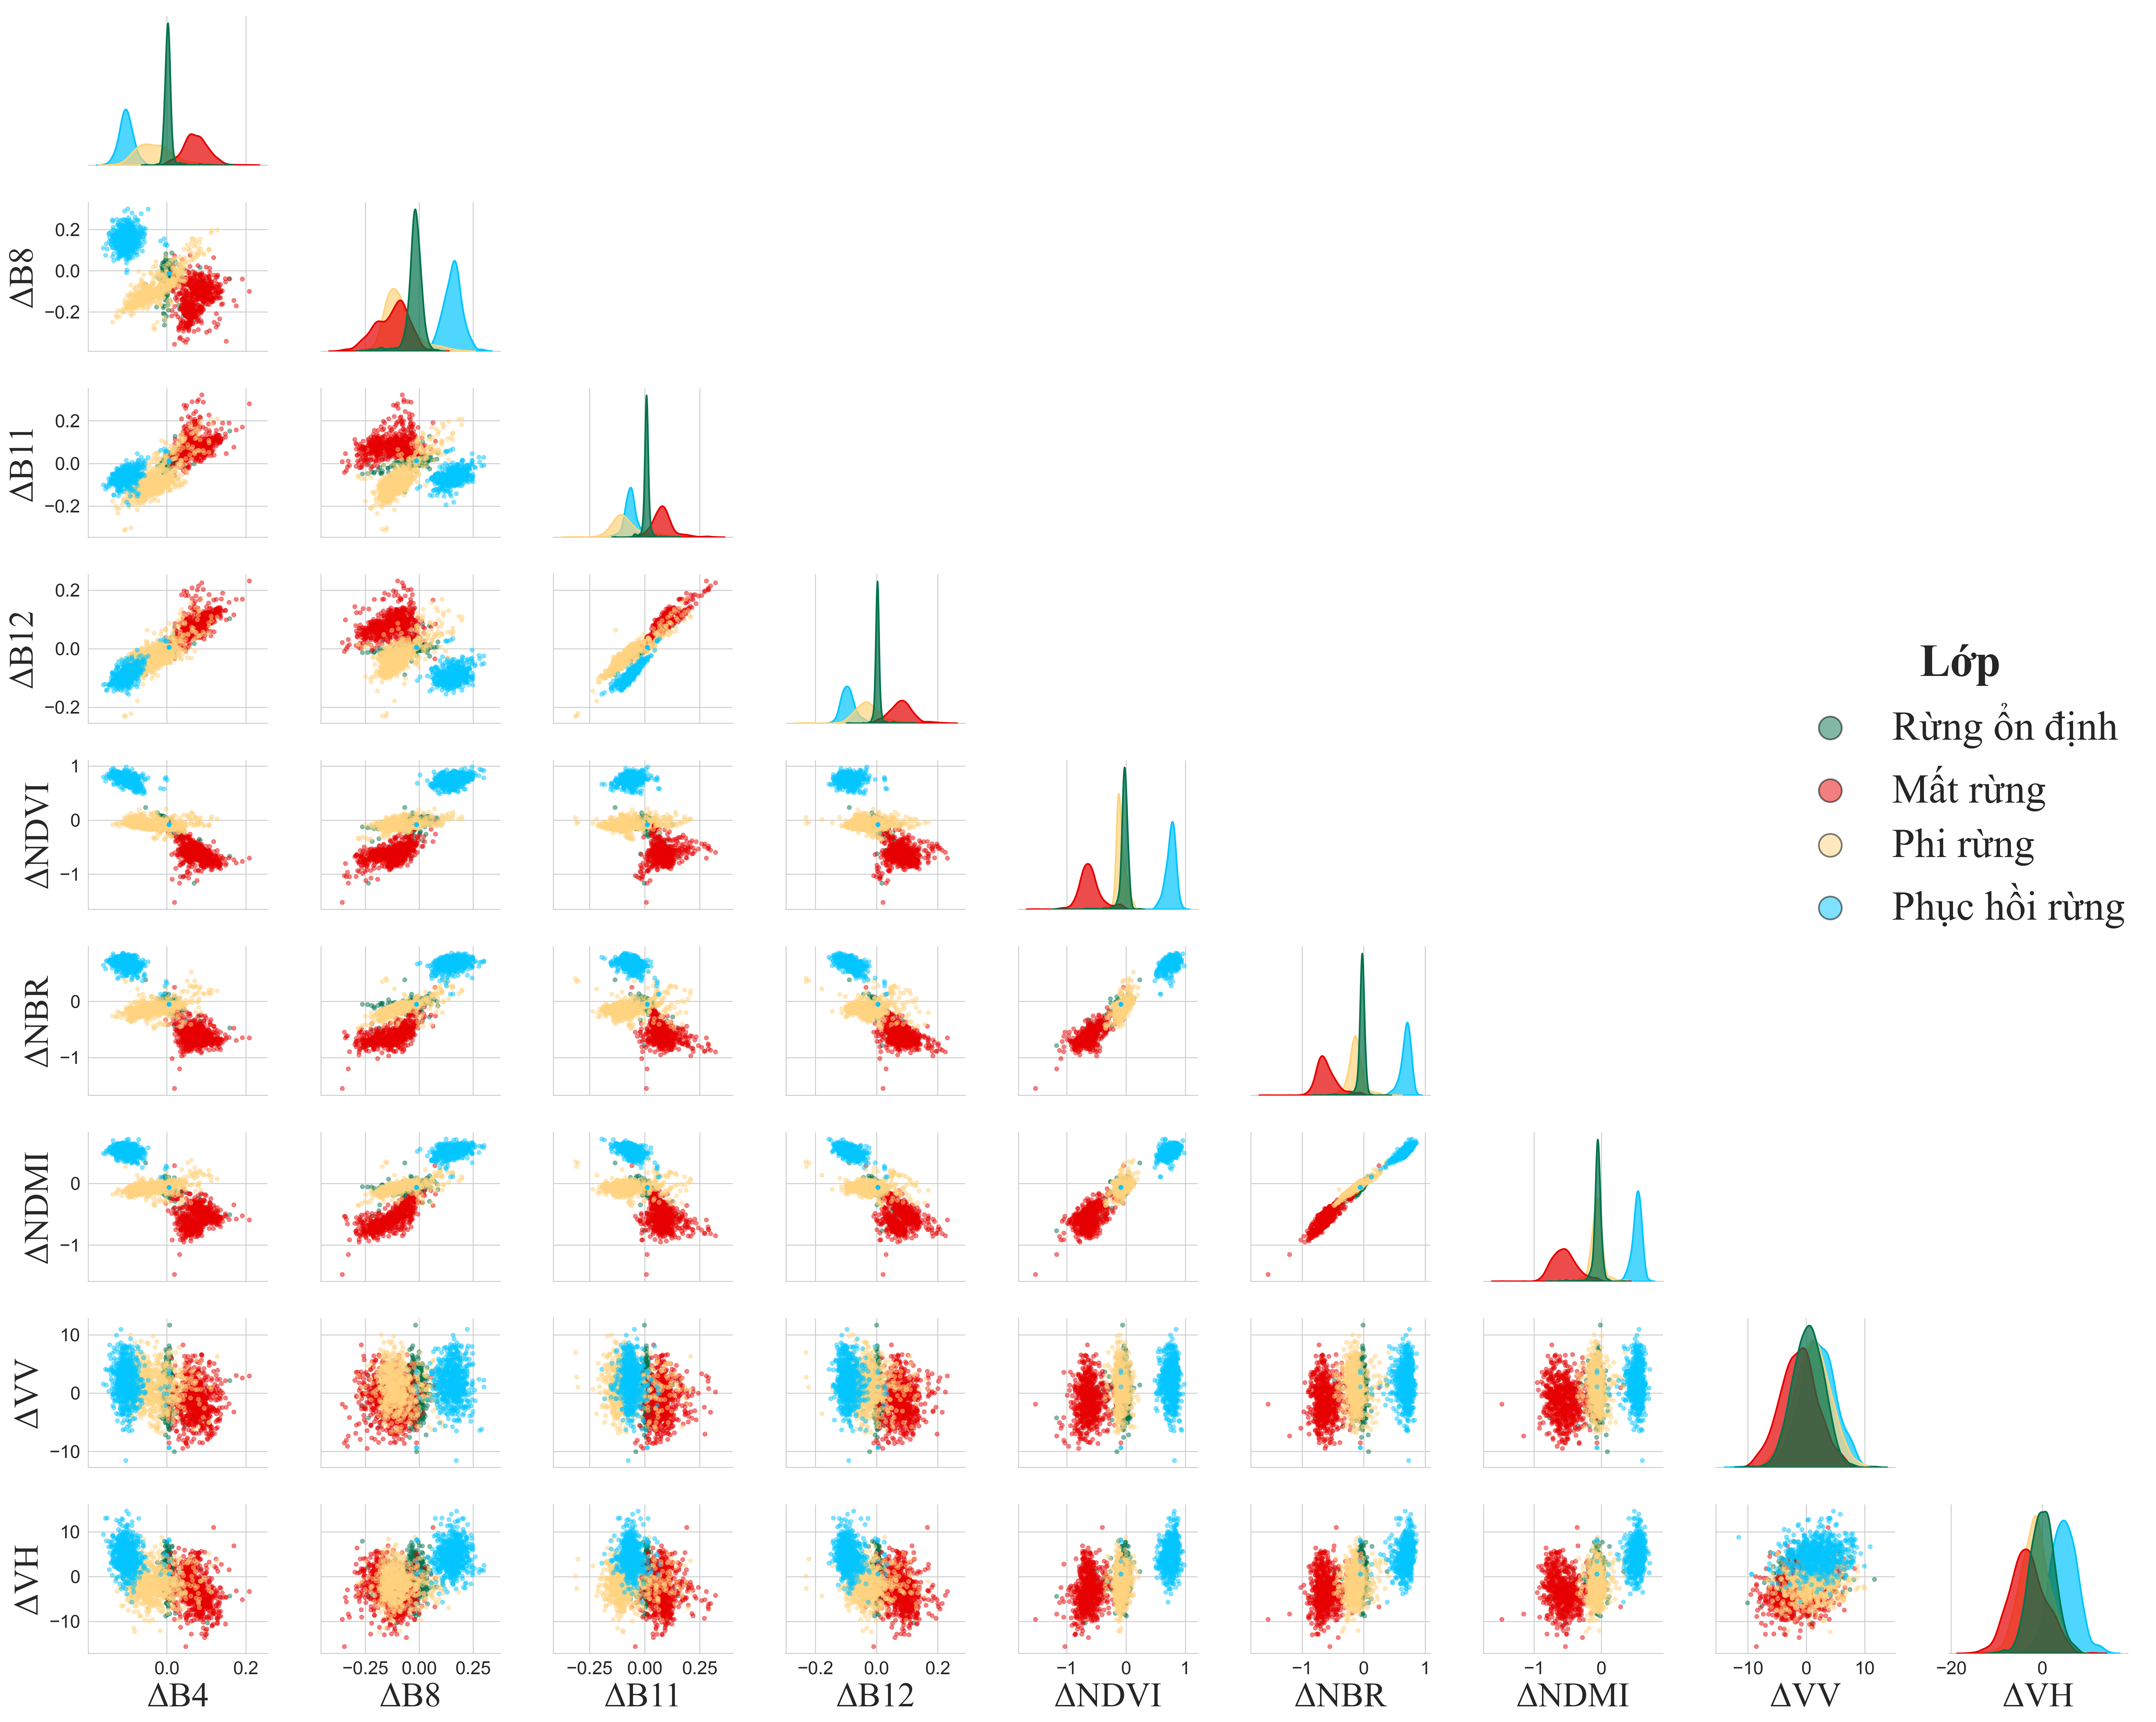
\includegraphics[width=0.95\textwidth]{img/chapter3/pairplot_delta_features.png}
\caption{Phân bố các đặc trưng delta theo lớp biến động rừng}
\label{fig:pairplot_delta}
\end{figure}

Biểu đồ trình bày mối quan hệ giữa 9 đặc trưng delta bao gồm các band quang phổ Sentinel-2 ($\Delta$B4, $\Delta$B8, $\Delta$B11, $\Delta$B12), các chỉ số thực vật ($\Delta$NDVI, $\Delta$NBR, $\Delta$NDMI) và các kênh ra-đa Sentinel-1 ($\Delta$VV, $\Delta$VH). Trên đường chéo chính, biểu đồ thể hiện phân bố của từng đặc trưng theo bốn lớp biến động; các ô còn lại hiển thị biểu đồ tán xạ giữa các cặp đặc trưng.

Phân tích phân bố trên đường chéo cho thấy các chỉ số thực vật delta thể hiện khả năng phân biệt vượt trội giữa các lớp biến động. Cụ thể, lớp Rừng ổn định và Phi rừng có phân bố tập trung quanh giá trị 0, phản ánh sự ổn định về lớp phủ thực vật qua hai thời điểm quan sát. Ngược lại, lớp Mất rừng thể hiện phân bố lệch về phía âm do sự suy giảm các chỉ số thực vật khi rừng bị chuyển đổi, trong khi lớp Phục hồi rừng có phân bố lệch về phía dương tương ứng với sự gia tăng sinh khối thực vật. Sự phân tách rõ ràng này khẳng định vai trò then chốt của $\Delta$NDVI, $\Delta$NBR và $\Delta$NDMI trong việc nhận diện biến động rừng.

Đối với các band quang phổ gốc, mức độ chồng chéo giữa các lớp cao hơn so với các chỉ số thực vật, tuy nhiên $\Delta$B8 (kênh cận hồng ngoại) vẫn cho thấy khả năng phân biệt tương đối tốt giữa lớp Mất rừng và Phục hồi rừng. Các đặc trưng ra-đa $\Delta$VV và $\Delta$VH có phân bố chồng chéo đáng kể giữa bốn lớp, cho thấy khả năng phân biệt độc lập hạn chế hơn so với dữ liệu quang học. Tuy nhiên, việc tích hợp dữ liệu ra-đa vẫn mang lại giá trị bổ sung, đặc biệt trong điều kiện mây che phủ thường xuyên tại khu vực nghiên cứu.

Phân tích các biểu đồ tán xạ cho thấy mối tương quan dương mạnh giữa ba chỉ số thực vật ($\Delta$NDVI, $\Delta$NBR, $\Delta$NDMI), thể hiện qua sự phân bố các điểm dữ liệu gần đường chéo. Tương tự, $\Delta$B11 và $\Delta$B12 có tương quan cao do cùng thuộc dải sóng ngắn hồng ngoại (SWIR). Trên không gian đặc trưng hai chiều của các chỉ số thực vật, lớp Mất rừng và Phục hồi rừng phân bố ở hai vùng đối lập nhau, trong khi lớp Rừng ổn định và Phi rừng tập trung quanh gốc tọa độ. Đặc điểm phân bố này tạo điều kiện thuận lợi cho mô hình CNN trong việc học các ranh giới quyết định phân tách bốn lớp biến động.

\subsection{Cấu hình phần cứng và phần mềm}

Môi trường thí nghiệm sử dụng phần cứng với CPU Intel Xeon E-2334 (4 nhân, 8 luồng), GPU NVIDIA GeForce RTX 4080 (16GB VRAM), bộ nhớ RAM 64GB và bộ nhớ lưu trữ 1TB SSD. Về phần mềm, hệ điều hành được sử dụng là Windows 10 Pro, môi trường Python 3.11 cùng PyTorch 2.5 có hỗ trợ CUDA 12.1 để huấn luyện mô hình, rasterio 1.4 (GDAL 3.6) cho xử lý dữ liệu không gian và các thư viện khoa học dữ liệu như NumPy, scikit-learn và pandas.

PyTorch được lựa chọn làm framework học sâu chính cho nghiên cứu này vì một số lý do. Thứ nhất, PyTorch sử dụng cơ chế đồ thị tính toán động (dynamic computational graph), cho phép xây dựng và sửa đổi kiến trúc mô hình một cách linh hoạt trong quá trình thử nghiệm. Thứ hai, cú pháp của PyTorch gần gũi với Python thuần túy, giúp việc triển khai và gỡ lỗi mô hình trở nên trực quan hơn. Thứ ba, PyTorch được hỗ trợ bởi cộng đồng nghiên cứu rộng lớn với nhiều mô hình tiền huấn luyện và thư viện mở rộng như torchvision, torchaudio. Cuối cùng, khả năng tích hợp tốt với CUDA cho phép tận dụng hiệu quả GPU trong quá trình huấn luyện và suy luận.

\subsection{Phân chia dữ liệu}

Bộ dữ liệu thực địa gồm 2.630 điểm, trong đó phân bố lớp gần như cân bằng: Lớp 0 (Rừng ổn định) 656 điểm (24,94\%), Lớp 1 (Mất rừng) 650 điểm (24,71\%), Lớp 2 (Phi rừng) 664 điểm (25,25\%) và Lớp 3 (Phục hồi rừng) 660 điểm (25,10\%).

\begin{table}[H]
\centering
\caption{Phân bố dữ liệu theo tập huấn luyện và kiểm tra}
\label{tab:data_split_info}
\begin{tabular}{|l|c|c|}
\hline
\textbf{Tập dữ liệu} & \textbf{Số mẫu} & \textbf{Tỷ lệ} \\
\hline
Huấn luyện + Kiểm định (5-Fold CV) & 2.104 & 80\% \\
\hline
Kiểm tra (cố định) & 526 & 20\% \\
\hline
\textbf{Tổng} & \textbf{2.630} & \textbf{100\%} \\
\hline
\end{tabular}
\end{table}

Việc chia tập dữ liệu được thực hiện như sau: 80\% dữ liệu (2.104 patches) được dành cho Huấn luyện + Kiểm định để thực hiện Kiểm định chéo 5 phần, còn 20\% dữ liệu (526 patches) được giữ lại làm tập dữ liệu kiểm tra cố định.

Kết quả trên hoàn thành mục tiêu thứ nhất, xây dựng bộ dữ liệu huấn luyện gồm 2.630 điểm mẫu với 27 đặc trưng từ ảnh vệ tinh Sentinel-1 và Sentinel-2 đa thời gian, bao gồm các kênh phổ, chỉ số thực vật và tán xạ ngược cho khu vực quy hoạch lâm nghiệp tỉnh Cà Mau.


% 3.2. Thử nghiệm mô hình
\section{Thử nghiệm mô hình}

\subsection{Ảnh hưởng của Patch Size}

\begin{table}[H]
\centering
\caption{So sánh các kích thước patch}
\label{tab:patch_size}
\begin{tabular}{|c|c|c|c|c|}
\hline
\textbf{Patch Size} & \textbf{Accuracy} & \textbf{ROC-AUC} & \textbf{Thời gian huấn luyện} & \textbf{Số tham số} \\
\hline
1×1 (pixel-wise) & 98.23\% & 99.78\% & 12.5s & 25,348 \\
\hline
\textbf{3×3 (baseline)} & \textbf{98.86\%} & \textbf{99.98\%} & 15.2s & 36,676 \\
\hline
5×5 & 98.67\% & 99.89\% & 28.3s & 52,484 \\
\hline
7×7 & 98.29\% & 99.86\% & 41.2s & 71,108 \\
\hline
\end{tabular}
\end{table}

\begin{figure}[H]
    \centering
    \begin{tikzpicture}
        \begin{axis}[
            ybar,
            width=0.85\textwidth,
            height=7cm,
            ylabel={Accuracy (\%)},
            xlabel={Patch Size},
            symbolic x coords={1x1, 3x3, 5x5, 7x7},
            xtick=data,
            ymin=97.5,
            ymax=99.5,
            bar width=25pt,
            nodes near coords,
            nodes near coords align={vertical},
            every node near coord/.append style={font=\scriptsize},
            enlarge x limits=0.2,
        ]
        \addplot[fill=blue!60] coordinates {
            (1x1, 98.23)
            (3x3, 98.86)
            (5x5, 98.67)
            (7x7, 98.29)
        };
        \end{axis}
    \end{tikzpicture}
    \caption{So sánh Accuracy theo các Patch Size}
    \label{fig:patch_size_comparison}
\end{figure}

Qua Bảng~\ref{tab:patch_size} và Hình~\ref{fig:patch_size_comparison}, có thể rút ra một số nhận xét quan trọng. Với patch size 1×1 (pixel-wise), mô hình đạt accuracy 98.23\%, cho thấy chỉ riêng thông tin phổ tại mỗi pixel đã đủ để phân biệt các lớp biến động rừng với độ chính xác cao, tuy nhiên cách tiếp cận này bỏ qua thông tin ngữ cảnh không gian. Patch size 3×3 đạt kết quả tốt nhất (98.86\% accuracy, 99.98\% ROC-AUC) với mức tăng thời gian huấn luyện chấp nhận được (+2.7 giây so với 1×1), cho thấy kích thước này cân bằng tốt giữa việc khai thác ngữ cảnh không gian địa phương và tránh nhiễu từ các pixel xa.

Đối với patch size 5×5 và 7×7, accuracy giảm dần (98.67\% và 98.29\%) mặc dù số tham số mô hình tăng đáng kể, cho thấy với độ phân giải 10m của Sentinel-2, ngữ cảnh không gian quá rộng (50-70m) có thể đưa vào nhiễu từ các lớp phủ lân cận, đặc biệt tại các vùng ranh giới. Thời gian huấn luyện tăng gần tuyến tính với số tham số, từ 12.5s (1×1) lên 41.2s (7×7), cho thấy chi phí tính toán tăng đáng kể khi mở rộng patch size mà không đem lại cải thiện về accuracy. Do đó, có thể kết luận rằng patch size 3×3 là tối ưu cho bộ dữ liệu này, đạt được sự cân bằng tốt nhất giữa độ chính xác, thời gian huấn luyện và khả năng khai thác ngữ cảnh không gian.

\subsection{Ảnh hưởng của nguồn dữ liệu}

\begin{table}[H]
\centering
\caption{Nghiên cứu loại trừ các nguồn dữ liệu}
\label{tab:data_sources}
\begin{tabular}{|l|c|c|c|}
\hline
\textbf{Cấu hình} & \textbf{Số đặc trưng} & \textbf{Accuracy} & \textbf{ROC-AUC} \\
\hline
Chỉ Sentinel-2 (delta) & 7 & 87.65\% & 94.12\% \\
\hline
Sentinel-2 (trước + sau + delta) & 21 & 93.42\% & 97.58\% \\
\hline
Chỉ Sentinel-1 (trước + sau + delta) & 6 & 83.27\% & 91.45\% \\
\hline
\textbf{S1 + S2 (tất cả)} & \textbf{27} & \textbf{98.86\%} & \textbf{99.98\%} \\
\hline
\end{tabular}
\end{table}

\begin{figure}[H]
    \centering
    \begin{tikzpicture}
        \begin{axis}[
            ybar,
            width=0.95\textwidth,
            height=7cm,
            ylabel={Accuracy (\%)},
            symbolic x coords={S2 (delta), S2 (tất cả), S1 (tất cả), S1+S2 (tất cả)},
            xtick=data,
            xticklabel style={rotate=15, anchor=east, font=\small},
            ymin=80,
            ymax=100,
            bar width=22pt,
            nodes near coords,
            nodes near coords align={vertical},
            every node near coord/.append style={font=\scriptsize},
            enlarge x limits=0.15,
        ]
        \addplot[fill=orange!70] coordinates {
            (S2 (delta), 87.65)
            (S2 (tất cả), 93.42)
            (S1 (tất cả), 83.27)
            (S1+S2 (tất cả), 98.86)
        };
        \end{axis}
    \end{tikzpicture}
    \caption{So sánh Accuracy theo các nguồn dữ liệu}
    \label{fig:data_sources_comparison}
\end{figure}

Qua Bảng~\ref{tab:data_sources} và Hình~\ref{fig:data_sources_comparison}, có thể rút ra các nhận xét quan trọng về vai trò của từng nguồn dữ liệu. Sentinel-2 đóng vai trò chủ đạo trong phân loại biến động rừng, thể hiện qua việc chỉ với dữ liệu Sentinel-2 delta (7 kênh biến động), mô hình đã đạt 87.65\% accuracy, và khi bổ sung đầy đủ dữ liệu trước, sau và delta (21 kênh), accuracy tăng lên 93.42\%, khẳng định tầm quan trọng của thông tin quang phổ và phương pháp phân tích 2 thời điểm trong phát hiện biến động. Trong khi đó, Sentinel-1 đơn lẻ có hiệu suất thấp nhất (83.27\% accuracy với 6 kênh); dữ liệu ra-đa khẩu độ tổng hợp tuy có ưu điểm không bị ảnh hưởng bởi mây và có khả năng quan sát cấu trúc rừng, nhưng độ phân giải phổ hạn chế (chỉ có VV và VH) khiến việc phân biệt các lớp phủ trở nên khó khăn hơn đáng kể so với dữ liệu quang học đa phổ.

Sự kết hợp S1+S2 cho kết quả tốt nhất (98.86\% accuracy, 99.98\% ROC-AUC), vượt trội đáng kể so với việc chỉ sử dụng Sentinel-2 (+5.44\%), cho thấy dữ liệu ra-đa bổ sung thông tin cấu trúc và độ ẩm mà dữ liệu quang học không nắm bắt được, đặc biệt hữu ích cho việc phân biệt rừng có mật độ tán khác nhau, phát hiện vùng rừng suy thoái chưa thể hiện rõ trên ảnh quang học, và cải thiện phân loại trong điều kiện có mây một phần. Bên cạnh đó, đóng góp của thông tin thời gian là đáng kể khi accuracy tăng từ 87.65\% (chỉ delta) lên 93.42\% (đầy đủ trước + sau + delta), khẳng định giá trị của việc khai thác thông tin đa thời gian trong phát hiện biến động.

Từ các kết quả trên, có thể kết luận rằng việc kết hợp Sentinel-1 và Sentinel-2 cho kết quả tối ưu nhất. Dữ liệu ra-đa và quang học có tính bổ sung cao: Sentinel-2 cung cấp thông tin chi tiết về thành phần hóa học và sinh lý của thực vật thông qua các kênh quang phổ, trong khi Sentinel-1 cung cấp thông tin về cấu trúc và độ ẩm của tán rừng. Sự kết hợp này đặc biệt phù hợp cho giám sát rừng ngập mặn ven biển, nơi điều kiện thời tiết thường xuyên có mây và sương mù.


% 3.3. Kết quả
\section{Kết quả}

\subsection{Kết quả huấn luyện mô hình CNN}

Để đánh giá độ ổn định của mô hình, nghiên cứu áp dụng phương pháp kiểm định chéo 5 phần. Phương pháp này chia dữ liệu thành 5 phần bằng nhau, luân phiên sử dụng mỗi phần làm tập kiểm tra trong khi 4 phần còn lại làm tập huấn luyện; kết quả cuối cùng là trung bình của 5 lần đánh giá. Bảng~\ref{tab:cv_training_summary} tổng hợp các thông số huấn luyện của 5 phần và Hình~\ref{fig:cv_comparison} so sánh Accuracy giữa các phần.

\begin{table}[H]
\centering
\caption{Tổng hợp kết quả huấn luyện kiểm định 5 phần}
\label{tab:cv_training_summary}
\begin{tabular}{|c|c|c|c|}
\hline
\textbf{Phần} & \textbf{Epoch tốt nhất} & \textbf{Loss cao nhất} & \textbf{Accuracy cao nhất} \\
\hline
Phần 1 & 59 & 0,0531 & 98,57\% \\
\hline
Phần 2 & 77 & 0,0401 & 99,05\% \\
\hline
Phần 3 & 82 & 0,0501 & 98,34\% \\
\hline
Phần 4 & 86 & 0,0683 & 98,10\% \\
\hline
Phần 5 & 50 & 0,0546 & 98,33\% \\
\hline
\textbf{Trung bình} & \textbf{71} & \textbf{0,0532} & \textbf{98,48\%} \\
\hline
\end{tabular}
\end{table}

\begin{figure}[H]
    \centering
    \begin{tikzpicture}
        \begin{axis}[
            ybar,
            width=0.85\textwidth,
            height=7cm,
            ylabel={Accuracy (\%)},
            xlabel={Phần kiểm định},
            symbolic x coords={Phần 1, Phần 2, Phần 3, Phần 4, Phần 5},
            xtick=data,
            ymin=97.5,
            ymax=100,
            bar width=20pt,
            nodes near coords,
            nodes near coords align={vertical},
            every node near coord/.append style={font=\scriptsize},
            enlarge x limits=0.15,
        ]
        \addplot[fill=blue!60] coordinates {
            (Phần 1, 98.57)
            (Phần 2, 99.05)
            (Phần 3, 98.34)
            (Phần 4, 98.10)
            (Phần 5, 98.33)
        };
        % Đường trung bình
        \addplot[red, thick, dashed, domain=0:5] coordinates {
            (Phần 1, 98.48) (Phần 2, 98.48) (Phần 3, 98.48) (Phần 4, 98.48) (Phần 5, 98.48)
        };
        \legend{Accuracy, Mean (98.48\%)}
        \end{axis}
    \end{tikzpicture}
    \caption{So sánh Accuracy giữa các phần kiểm định trong kiểm định chéo 5 phần}
    \label{fig:cv_comparison}
\end{figure}

Qua Hình~\ref{fig:cv_comparison}, Accuracy dao động trong khoảng hẹp từ 98,10\% đến 99,05\%, biên độ chênh lệch chỉ 0,95 điểm phần trăm. Kết quả kiểm định chéo cho thấy mô hình đạt độ ổn định cao với độ lệch chuẩn 0,36\%. Accuracy của từng phần kiểm định đều vượt ngưỡng 98\%, phản ánh khả năng tổng quát hóa tốt. Hiện tượng loss kiểm định thấp hơn loss huấn luyện là đặc trưng điển hình khi sử dụng Dropout tỷ lệ cao (70\%), cho thấy kỹ thuật điều chuẩn hoạt động hiệu quả và mô hình không bị quá khớp. Cơ chế dừng sớm đã dừng huấn luyện tại các epoch khác nhau cho mỗi phần kiểm định (từ epoch 50 đến 86), xác nhận mô hình đã hội tụ tốt.

Sau khi hoàn tất kiểm định chéo, mô hình cuối cùng được huấn luyện trên toàn bộ 80\% dữ liệu (2.104 mẫu) để tận dụng tối đa lượng dữ liệu huấn luyện. Hình~\ref{fig:final_training} trình bày diễn biến loss và accuracy trong quá trình huấn luyện.

\begin{figure}[H]
\centering
\includegraphics[width=0.95\textwidth]{img/chapter3/cnn_training_history.png}
\caption{Diễn biến loss và accuracy trong quá trình huấn luyện mô hình cuối cùng}
\label{fig:final_training}
\end{figure}

Quá trình huấn luyện kéo dài khoảng 70 epoch với loss giảm từ 1,8 xuống 0,2 và accuracy tăng từ 30\% lên trên 95\%. Mô hình này sau đó được đánh giá trên 20\% tập kiểm tra cố định (526 mẫu) để báo cáo kết quả cuối cùng.

Trên tập kiểm tra, mô hình đạt Accuracy 98,86\%, ROC-AUC 99,98\%, với Precision, Recall và F1-Score (macro average --- trung bình không trọng số từ mỗi lớp) đều đạt 98,86\%. Ma trận nhầm lẫn (Hình~\ref{fig:confusion_heatmap}) thể hiện kết quả phân loại, mỗi hàng tương ứng với lớp thực tế và mỗi cột tương ứng với lớp dự đoán; phần tử trên đường chéo chính là số mẫu phân loại đúng, phần tử ngoài đường chéo là trường hợp phân loại sai. Bảng~\ref{tab:class_analysis} trình bày các chỉ số đánh giá theo từng lớp.

\begin{figure}[H]
    \centering
    \begin{tikzpicture}
        % Định nghĩa màu sắc Blues colormap (từ nhạt đến đậm)
        \definecolor{blue0}{RGB}{247,251,255}
        \definecolor{blue1}{RGB}{222,235,247}
        \definecolor{blue2}{RGB}{198,219,239}
        \definecolor{blue3}{RGB}{158,202,225}
        \definecolor{blue4}{RGB}{107,174,214}
        \definecolor{blue5}{RGB}{66,146,198}
        \definecolor{blue6}{RGB}{33,113,181}
        \definecolor{blue7}{RGB}{8,81,156}
        \definecolor{blue8}{RGB}{8,48,107}

        % Kích thước ô
        \def\cellsize{1.8}

        % Vẽ các ô với màu Blues gradient
        % Hàng 0 (Rừng ổn định): 129, 2, 0, 0
        \fill[blue8] (0*\cellsize, 3*\cellsize) rectangle (1*\cellsize, 4*\cellsize);
        \fill[blue1] (1*\cellsize, 3*\cellsize) rectangle (2*\cellsize, 4*\cellsize);
        \fill[blue0] (2*\cellsize, 3*\cellsize) rectangle (3*\cellsize, 4*\cellsize);
        \fill[blue0] (3*\cellsize, 3*\cellsize) rectangle (4*\cellsize, 4*\cellsize);

        % Hàng 1 (Mất rừng): 4, 126, 0, 0
        \fill[blue1] (0*\cellsize, 2*\cellsize) rectangle (1*\cellsize, 3*\cellsize);
        \fill[blue8] (1*\cellsize, 2*\cellsize) rectangle (2*\cellsize, 3*\cellsize);
        \fill[blue0] (2*\cellsize, 2*\cellsize) rectangle (3*\cellsize, 3*\cellsize);
        \fill[blue0] (3*\cellsize, 2*\cellsize) rectangle (4*\cellsize, 3*\cellsize);

        % Hàng 2 (Phi rừng): 0, 0, 133, 0
        \fill[blue0] (0*\cellsize, 1*\cellsize) rectangle (1*\cellsize, 2*\cellsize);
        \fill[blue0] (1*\cellsize, 1*\cellsize) rectangle (2*\cellsize, 2*\cellsize);
        \fill[blue8] (2*\cellsize, 1*\cellsize) rectangle (3*\cellsize, 2*\cellsize);
        \fill[blue0] (3*\cellsize, 1*\cellsize) rectangle (4*\cellsize, 2*\cellsize);

        % Hàng 3 (Phục hồi rừng): 0, 0, 0, 132
        \fill[blue0] (0*\cellsize, 0*\cellsize) rectangle (1*\cellsize, 1*\cellsize);
        \fill[blue0] (1*\cellsize, 0*\cellsize) rectangle (2*\cellsize, 1*\cellsize);
        \fill[blue0] (2*\cellsize, 0*\cellsize) rectangle (3*\cellsize, 1*\cellsize);
        \fill[blue8] (3*\cellsize, 0*\cellsize) rectangle (4*\cellsize, 1*\cellsize);

        % Vẽ đường viền cho các ô
        \draw[white, line width=1pt] (0,0) grid[step=\cellsize] (4*\cellsize, 4*\cellsize);

        % Thêm số liệu vào các ô
        \node[font=\normalsize\bfseries, text=white] at (0.5*\cellsize, 3.5*\cellsize) {129};
        \node[font=\normalsize, text=black] at (1.5*\cellsize, 3.5*\cellsize) {2};
        \node[font=\normalsize, text=black] at (2.5*\cellsize, 3.5*\cellsize) {0};
        \node[font=\normalsize, text=black] at (3.5*\cellsize, 3.5*\cellsize) {0};

        \node[font=\normalsize, text=black] at (0.5*\cellsize, 2.5*\cellsize) {4};
        \node[font=\normalsize\bfseries, text=white] at (1.5*\cellsize, 2.5*\cellsize) {126};
        \node[font=\normalsize, text=black] at (2.5*\cellsize, 2.5*\cellsize) {0};
        \node[font=\normalsize, text=black] at (3.5*\cellsize, 2.5*\cellsize) {0};

        \node[font=\normalsize, text=black] at (0.5*\cellsize, 1.5*\cellsize) {0};
        \node[font=\normalsize, text=black] at (1.5*\cellsize, 1.5*\cellsize) {0};
        \node[font=\normalsize\bfseries, text=white] at (2.5*\cellsize, 1.5*\cellsize) {133};
        \node[font=\normalsize, text=black] at (3.5*\cellsize, 1.5*\cellsize) {0};

        \node[font=\normalsize, text=black] at (0.5*\cellsize, 0.5*\cellsize) {0};
        \node[font=\normalsize, text=black] at (1.5*\cellsize, 0.5*\cellsize) {0};
        \node[font=\normalsize, text=black] at (2.5*\cellsize, 0.5*\cellsize) {0};
        \node[font=\normalsize\bfseries, text=white] at (3.5*\cellsize, 0.5*\cellsize) {132};

        % Nhãn cột (Dự đoán) - xoay nghiêng
        \node[font=\scriptsize, rotate=45, anchor=east] at (0.5*\cellsize, -0.2*\cellsize) {Rừng ổn định};
        \node[font=\scriptsize, rotate=45, anchor=east] at (1.5*\cellsize, -0.2*\cellsize) {Mất rừng};
        \node[font=\scriptsize, rotate=45, anchor=east] at (2.5*\cellsize, -0.2*\cellsize) {Phi rừng};
        \node[font=\scriptsize, rotate=45, anchor=east] at (3.5*\cellsize, -0.2*\cellsize) {Phục hồi rừng};
        \node[font=\small\bfseries] at (2*\cellsize, -1.1*\cellsize) {Dự đoán};

        % Nhãn hàng (Thực tế)
        \node[font=\scriptsize, anchor=east] at (-0.1*\cellsize, 3.5*\cellsize) {Rừng ổn định};
        \node[font=\scriptsize, anchor=east] at (-0.1*\cellsize, 2.5*\cellsize) {Mất rừng};
        \node[font=\scriptsize, anchor=east] at (-0.1*\cellsize, 1.5*\cellsize) {Phi rừng};
        \node[font=\scriptsize, anchor=east] at (-0.1*\cellsize, 0.5*\cellsize) {Phục hồi rừng};
        \node[font=\small\bfseries, rotate=90] at (-1.5*\cellsize, 2*\cellsize) {Thực tế};

        % Thanh màu (color bar) - Blues gradient (9 segments, mỗi segment = 4/9 cellsize)
        \pgfmathsetmacro{\segheight}{4/9}
        \foreach \i/\col in {0/blue0, 1/blue1, 2/blue2, 3/blue3, 4/blue4, 5/blue5, 6/blue6, 7/blue7, 8/blue8} {
            \fill[\col] (5*\cellsize, \i*\segheight*\cellsize) rectangle (5.4*\cellsize, \i*\segheight*\cellsize+\segheight*\cellsize);
        }
        \draw[black, thin] (5*\cellsize, 0) rectangle (5.4*\cellsize, 4*\cellsize);
        \node[font=\tiny, anchor=west] at (5.5*\cellsize, 0) {0};
        \node[font=\tiny, anchor=west] at (5.5*\cellsize, 1*\cellsize) {40};
        \node[font=\tiny, anchor=west] at (5.5*\cellsize, 2*\cellsize) {80};
        \node[font=\tiny, anchor=west] at (5.5*\cellsize, 3*\cellsize) {120};
    \end{tikzpicture}
    \caption{Ma trận nhầm lẫn trên tập kiểm tra (n=526, Accuracy: 98,86\%)}
    \label{fig:confusion_heatmap}
\end{figure}

\begin{table}[H]
\centering
\caption{Phân tích chi tiết từng lớp}
\label{tab:class_analysis}
\begin{tabular}{|l|c|c|c|c|c|}
\hline
\textbf{Lớp} & \textbf{Precision} & \textbf{Recall} & \textbf{F1-Score} & \textbf{Số mẫu} & \textbf{Lỗi} \\
\hline
0 - Rừng ổn định & 96,99\% & 98,47\% & 97,73\% & 131 & 4 FP, 2 FN \\
\hline
1 - Mất rừng & 98,44\% & 96,92\% & 97,67\% & 130 & 2 FP, 4 FN \\
\hline
2 - Phi rừng & 100,00\% & 100,00\% & 100,00\% & 133 & 0 \\
\hline
3 - Phục hồi rừng & 100,00\% & 100,00\% & 100,00\% & 132 & 0 \\
\hline
\end{tabular}
\end{table}

Tổng cộng chỉ có 6/526 mẫu bị phân loại sai, tương đương tỷ lệ lỗi 1,14\%. Trong đó, hai mẫu thuộc Lớp 0 (Rừng ổn định) bị nhầm thành Lớp 1 (Mất rừng) và bốn mẫu thuộc Lớp 1 (Mất rừng) bị nhầm thành Lớp 0 (Rừng ổn định). Đánh giá chi tiết cho thấy Lớp 2 (Phi rừng) và Lớp 3 (Phục hồi rừng) được phân loại hoàn hảo với Accuracy 100\%.

Việc nhầm lẫn chỉ xảy ra giữa hai lớp Rừng ổn định (Lớp 0) và Mất rừng (Lớp 1) có thể được giải thích bởi một số yếu tố. Trước hết, cả hai lớp đều có sự hiện diện của rừng ở ít nhất một thời điểm, dẫn đến sự tương đồng về đặc trưng quang phổ; các khu vực rừng bị suy thoái nhẹ có thể có phổ phản xạ đặc trưng tương tự với rừng ổn định, đặc biệt khi mức độ mất rừng không rõ ràng. Bên cạnh đó, hiệu ứng biên cũng góp phần gây nhầm lẫn khi tại ranh giới giữa vùng rừng và vùng mất rừng, các điểm ảnh có thể chứa cả hai loại lớp phủ (điểm ảnh hỗn hợp), dẫn đến vector đặc trưng không điển hình cho một lớp cụ thể. Ngoài ra, một số khu vực rừng ngập mặn có thể có biến động theo mùa về mật độ tán lá, tạo ra sự thay đổi NDVI tương tự như mất rừng nhưng thực tế là biến động tự nhiên. Cuối cùng, với chỉ hai thời điểm quan sát, hạn chế về độ phân giải thời gian khiến một số biến động ngắn hạn hoặc phục hồi nhanh có thể không được ghi nhận chính xác.

Tuy nhiên, với tỷ lệ nhầm lẫn rất thấp (chỉ 6/526 mẫu, ~1,14\%) và ROC-AUC trung bình đạt 99,98\%, mô hình thể hiện khả năng phân biệt xuất sắc giữa các lớp biến động rừng.

\subsection{Kết quả phân loại toàn bộ vùng nghiên cứu}

Sau khi huấn luyện và đánh giá trên tập kiểm tra, mô hình được áp dụng để phân loại toàn bộ vùng quy hoạch lâm nghiệp tỉnh Cà Mau. Kết quả thống kê phân loại được trình bày trong Bảng~\ref{tab:area_distribution}.

\begin{table}[H]
\centering
\caption{Phân bố diện tích theo lớp phân loại}
\label{tab:area_distribution}
\begin{tabular}{|c|l|r|r|r|r|}
\hline
\textbf{Lớp} & \textbf{Tên lớp} & \textbf{Số điểm ảnh} & \textbf{Tỷ lệ (\%)} & \textbf{Diện tích (ha)} & \textbf{Diện tích (km²)} \\
\hline
0 & Rừng ổn định & 12.071.691 & 74,30\% & 120.716,91 & 1.207,17 \\
\hline
1 & Mất rừng & 728.215 & 4,48\% & 7.282,15 & 72,82 \\
\hline
2 & Phi rừng & 2.952.854 & 18,17\% & 29.528,54 & 295,29 \\
\hline
3 & Phục hồi rừng & 494.090 & 3,04\% & 4.940,90 & 49,41 \\
\hline
\textbf{Tổng} & & \textbf{16.246.850} & \textbf{100\%} & \textbf{162.468,50} & \textbf{1.624,69} \\
\hline
\end{tabular}
\end{table}

Kết quả từ Bảng~\ref{tab:area_distribution} cho thấy bức tranh tổng quan về tình trạng biến động rừng tại tỉnh Cà Mau trong giai đoạn nghiên cứu. Lớp rừng ổn định chiếm tỷ lệ lớn nhất với 74,30\% (tương đương 1.207,17 km²), phản ánh nỗ lực bảo tồn và quản lý rừng ngập mặn của địa phương, chủ yếu tập trung tại Vườn Quốc gia Mũi Cà Mau và các vùng đệm được bảo vệ nghiêm ngặt. Diện tích mất rừng chiếm 4,48\% (72,82 km²), đây là tỷ lệ đáng quan ngại khi quy đổi ra diện tích tuyệt đối, với các nguyên nhân chính có thể bao gồm chuyển đổi mục đích sử dụng đất sang nuôi trồng thủy sản, xói lở bờ biển do biến đổi khí hậu và tác động của xâm nhập mặn làm suy thoái rừng.

Lớp phi rừng chiếm 18,17\% (295,29 km²), bao gồm các khu vực ao nuôi tôm, đất trống, khu dân cư và cơ sở hạ tầng, phản ánh áp lực phát triển kinh tế - xã hội lên tài nguyên rừng trong khu vực. Lớp phục hồi rừng chiếm 3,04\% (49,41 km²), cho thấy một phần diện tích đã được tái sinh tự nhiên hoặc trồng rừng mới. Mặc dù tỷ lệ phục hồi còn thấp hơn so với diện tích mất rừng, đây vẫn là tín hiệu tích cực cho công tác phục hồi hệ sinh thái rừng ngập mặn trong khu vực. Hình~\ref{fig:classification_map} minh họa sự phân bố không gian của các lớp phân loại trên toàn vùng nghiên cứu.

\begin{figure}[H]
    \centering
    \includegraphics[width=0.95\textwidth]{img/chapter3/Classification.png}
    \caption{Bản đồ phân loại biến động rừng tỉnh Cà Mau}
    \label{fig:classification_map}
\end{figure}

Để phân tích chi tiết hơn về khả năng phát hiện biến động của mô hình trong điều kiện thực tế, nghiên cứu lựa chọn khu vực Vườn Quốc gia Mũi Cà Mau làm ví dụ minh họa. Đây là khu vực đặc trưng với sự đan xen giữa rừng ngập mặn nguyên sinh, hệ thống ao nuôi tôm và các hoạt động sản xuất theo mô hình Tôm--Rừng, tạo nên bức tranh đa dạng về các loại biến động lớp phủ.

\begin{figure}[H]
    \centering
    \includegraphics[width=0.95\textwidth]{img/chapter3/VQG_Mui_Ca_Mau.png}
    \caption{Bản đồ phân loại biến động rừng khu vực Vườn Quốc gia Mũi Cà Mau}
    \label{fig:vqg_mui_ca_mau}
\end{figure}

Kết quả phân loại biến động rừng ngập mặn khu vực Vườn Quốc gia Mũi Cà Mau (Hình~\ref{fig:vqg_mui_ca_mau}) cho thấy mô hình có khả năng nhận diện chính xác một số loại biến động thực sự của lớp phủ. Các vùng mất rừng (màu đỏ) phân bố chủ yếu dọc theo rìa ao nuôi và hệ thống kênh mương, phản ánh các hoạt động sản xuất như mở rộng diện tích ao tôm, nạo vét mương, cải tạo bờ bao hoặc phơi ao. Tại những khu vực này, việc dọn cây đã làm suy giảm rõ rệt thảm thực vật và để lộ lớp đất hoặc bùn bên dưới --- đây là những biến động thực sự mà mô hình phát hiện hợp lý. Tương tự, các vùng phục hồi rừng (màu xanh lam) xuất hiện rải rác ven bờ ao và trong các khoảng trống nhỏ, đặc biệt dọc theo đường bờ biển, phản ánh quá trình tái sinh tự nhiên của cây ngập mặn non trong hệ sinh thái Tôm--Rừng.

Tuy nhiên, kết quả phân loại cũng chứa đựng những sai số tiềm ẩn do các yếu tố môi trường gây nhiễu. Thủy triều là nguồn gây nhiễu đáng kể: khi triều cường, các mảng rừng thấp bị ngập tạm thời có thể bị phân loại nhầm thành mất rừng; ngược lại, khi triều kiệt, sự xuất hiện của bãi bùn và thảm thực vật thấp có thể tạo ra tín hiệu giả của phục hồi rừng. Bên cạnh đó, hoạt động nuôi tôm cũng góp phần tạo ra các biến động ``ảo'' khi ao nuôi thường xuyên thay nước, mực nước và độ đục dao động liên tục khiến đặc trưng phổ của mặt nước thay đổi giữa hai thời điểm thu ảnh. Trong mùa khô, hiện tượng ao cạn đáy hoặc bùn bị phơi tự nhiên cũng có thể dẫn đến phân loại sai thành mất rừng mặc dù không có tác động sinh thái thực sự.

Tóm lại, mô hình thể hiện khả năng mô tả tương đối chính xác các biến động liên quan đến hoạt động sản xuất và tái sinh rừng ngập mặn, song độ tin cậy giảm đáng kể tại các khu vực nhạy cảm với biến động môi trường --- đặc biệt là những nơi rừng thấp, gần mép ao hoặc chịu ảnh hưởng mạnh của chế độ thủy triều và hoạt động nuôi trồng thủy sản.

\begin{figure}[H]
    \centering
    \definecolor{stableforest}{HTML}{00734C}
    \definecolor{deforestation}{HTML}{E60000}
    \definecolor{nonforest}{HTML}{FFD37F}
    \definecolor{reforestation}{HTML}{00C5FF}
    \begin{tikzpicture}
        \pie[
            radius=3,
            text=legend,
            color={stableforest, deforestation, nonforest, reforestation},
            explode={0, 0.1, 0, 0}
        ]{
            74.30/Rừng ổn định (74{,}30\%),
            4.48/Mất rừng (4{,}48\%),
            18.17/Phi rừng (18{,}17\%),
            3.04/Phục hồi rừng (3{,}04\%)
        }
    \end{tikzpicture}
    \caption{Tỷ lệ diện tích các lớp phân loại}
    \label{fig:pie_chart}
\end{figure}

Qua biểu đồ tròn (Hình~\ref{fig:pie_chart}), có thể nhận thấy sự chênh lệch rõ rệt về diện tích giữa các lớp. Rừng ổn định chiếm ưu thế tuyệt đối với hơn 3/4 diện tích vùng nghiên cứu. Đáng chú ý, tỷ lệ mất rừng (4,48\%) vượt quá tỷ lệ phục hồi rừng (3,04\%), cho thấy xu hướng suy giảm ròng của diện tích rừng trong giai đoạn nghiên cứu, với chênh lệch khoảng 1,44\% (tương đương 2.341 ha) là mức độ mất rừng ròng mà khu vực đang phải đối mặt. Tuy nhiên, cần lưu ý rằng việc khai thác rừng trồng (hợp pháp) có tính chu kỳ, nên vào thời điểm sau khai thác diện tích rừng tuyệt đối có thể giảm tạm thời; điều này không nhất thiết phản ánh xu hướng mất rừng dài hạn của khu vực. Diện tích phi rừng lớn (18,17\%) phản ánh mức độ khai thác tài nguyên đất đai trong khu vực, chủ yếu cho hoạt động nuôi trồng thủy sản - ngành kinh tế mũi nhọn của tỉnh Cà Mau.

Cần lưu ý rằng theo khuyến nghị của Olofsson và cộng sự \citeen{olofsson2014}, diện tích ước tính từ bản đồ phân loại cần được hiệu chỉnh dựa trên Ma trận nhầm lẫn để đảm bảo tính không chệch. Với Accuracy cao của mô hình (98,86\%, Precision và Recall đều trên 96\% cho tất cả các lớp), sai số giữa diện tích thô và diện tích hiệu chỉnh được kỳ vọng là nhỏ.  Việc thực hiện hiệu chỉnh đầy đủ theo phương pháp Olofsson sẽ là hướng phát triển trong tương lai.

Kết quả trên hoàn thành mục tiêu thứ tư, áp dụng mô hình CNN đã huấn luyện để phân loại biến động rừng toàn vùng quy hoạch lâm nghiệp tỉnh Cà Mau (162.468,50 ha) và tạo bản đồ biến động ở độ phân giải 10m với 4 lớp phân loại.

\subsection{So sánh với các nghiên cứu khác}

Việc so sánh trực tiếp các chỉ số đánh giá giữa các nghiên cứu khác nhau có những hạn chế nhất định. Sự khác biệt về đặc điểm sinh thái của khu vực nghiên cứu (rừng ngập mặn ven biển so với rừng nhiệt đới nội địa), độ phân giải không gian của dữ liệu đầu vào (Sentinel-2 10m so với Landsat 30m), quy mô và phương pháp thu thập dữ liệu tham chiếu, cùng với định nghĩa các lớp phân loại có thể dẫn đến những khác biệt đáng kể về kết quả đánh giá. Do vậy, các so sánh được trình bày dưới đây nhằm mục đích định vị phương pháp đề xuất trong bối cảnh phát triển chung của lĩnh vực, thay vì đưa ra kết luận về tính ưu việt tuyệt đối.

Để đánh giá hiệu quả của phương pháp đề xuất, kết quả được so sánh với các công trình nghiên cứu tiêu biểu trong lĩnh vực giám sát biến động rừng bằng viễn thám và học máy. Nghiên cứu của Hansen và cộng sự \citeen{hansen2013} tại Đại học Maryland là công trình tiên phong trong việc xây dựng bản đồ biến động rừng toàn cầu sử dụng ảnh Landsat 30m. Phương pháp sử dụng thuật toán Decision Trees kết hợp với nền tảng Google Earth Engine để xử lý hơn 654.000 cảnh Landsat 7 trong giai đoạn 2000--2012. Kết quả đánh giá độc lập cho thấy bản đồ mất rừng đạt tỷ lệ dương tính giả 13\% và âm tính giả 12\% ở quy mô toàn cầu, tương đương Accuracy khoảng 85\%. Phương pháp này có ưu điểm về quy mô toàn cầu, cập nhật hàng năm, miễn phí và công khai; tuy nhiên, nhược điểm là độ phân giải thấp (30m) khiến khó phát hiện biến động nhỏ, chỉ sử dụng dữ liệu quang học nên bị hạn chế bởi mây, và định nghĩa ``rừng'' dựa trên độ cao cây (>5m) không phù hợp với rừng ngập mặn non.

Trong những năm gần đây, các kiến trúc học sâu như CNN, U-Net và ResNet đã được áp dụng rộng rãi cho bài toán phát hiện biến động rừng với kết quả vượt trội so với phương pháp học máy truyền thống. Theo tổng quan của Fayaz và cộng sự (2024), U-Net và các biến thể của nó được sử dụng trong 45\% các nghiên cứu về phát hiện mất rừng, đạt Accuracy trung bình 94--97\%. Nghiên cứu của Ortega và cộng sự (2020) trên rừng Amazon cho thấy các kiến trúc CNN (SharpMask, U-Net, ResU-Net) đều vượt trội so với thuật toán ML truyền thống cả về định lượng lẫn trực quan. Đặc biệt, việc kết hợp U-Net với ResNet (ResU-Net) giúp trích xuất đặc trưng chi tiết hơn. Ưu điểm của học sâu là tự động học đặc trưng từ dữ liệu mà không cần thiết kế thủ công, khai thác được ngữ cảnh không gian và hiệu quả cao khi có đủ dữ liệu huấn luyện; tuy nhiên, nhược điểm là yêu cầu lượng dữ liệu huấn luyện lớn, tính chất ``hộp đen'' khó giải thích, chi phí tính toán cao và hiệu suất giảm đáng kể khi kích thước mẫu nhỏ.

Bảng~\ref{tab:comparison} tổng hợp kết quả so sánh giữa nghiên cứu này với các công trình tiêu biểu.

\begin{table}[H]
\centering
\caption{So sánh với các nghiên cứu trong tài liệu}
\label{tab:comparison}
\begin{tabular}{|l|l|l|c|c|}
\hline
\textbf{Nghiên cứu} & \textbf{Phương pháp} & \textbf{Dữ liệu} & \textbf{Accuracy} & \textbf{ROC-AUC} \\
\hline
Hansen và cs. (2013) & Decision Trees & Landsat 30m & $\sim$85\% & - \\
\hline
Ortega và cs. (2020) & U-Net, ResU-Net & Landsat 30m & $\sim$94\% & - \\
\hline
Fayaz và cs. (2024) & U-Net (tổng quan) & Đa nguồn & 94--97\% & - \\
\hline
\textbf{Nghiên cứu này} & \textbf{CNN (custom)} & \textbf{S1/S2 10m} & \textbf{98,86\%} & \textbf{99,98\%} \\
\hline
\end{tabular}
\end{table}

\begin{figure}[H]
    \centering
    \begin{tikzpicture}
        \begin{axis}[
            ybar,
            width=0.9\textwidth,
            height=7cm,
            ylabel={Accuracy (\%)},
            symbolic x coords={Hansen (2013), Ortega (2020), Fayaz (2024), Nghiên cứu này},
            xtick=data,
            xticklabel style={rotate=15, anchor=east, font=\small},
            ymin=80,
            ymax=102,
            bar width=25pt,
            nodes near coords,
            nodes near coords align={vertical},
            every node near coord/.append style={font=\scriptsize},
            enlarge x limits=0.15,
        ]
        \addplot[fill=teal!60] coordinates {
            (Hansen (2013), 85)
            (Ortega (2020), 94)
            (Fayaz (2024), 95.5)
            (Nghiên cứu này, 98.86)
        };
        \end{axis}
    \end{tikzpicture}
    \caption{So sánh Accuracy với các nghiên cứu trước đó}
    \label{fig:literature_comparison}
\end{figure}

Kết quả của nghiên cứu này đạt Accuracy cao hơn so với các công trình trước đó \citeen{stehman2019}. Hiệu suất này có thể được giải thích bởi độ phân giải không gian cao hơn (10m so với 30m) giúp phát hiện biến động chi tiết hơn, sự kết hợp dữ liệu đa nguồn (ra-đa và quang học) bổ sung cho nhau trong điều kiện nhiều mây của vùng nhiệt đới, kiến trúc CNN được thiết kế phù hợp với bộ dữ liệu nhỏ thông qua kỹ thuật điều chuẩn (Dropout 70\%, chuẩn hóa theo lô), cùng với bộ dữ liệu thực địa chất lượng cao được thu thập và kiểm tra kỹ lưỡng.

Nghiên cứu cũng thực hiện so sánh định tính với sản phẩm Giám sát rừng toàn cầu (Global Forest Watch - GFW) dựa trên công trình của Hansen và cộng sự đã đề cập ở trên, được cập nhật liên tục bởi Potapov và cộng sự \citeen{potapov2022}.

\begin{table}[H]
\centering
\caption{So sánh kết quả với Giám sát rừng toàn cầu (GFW)}
\label{tab:gfw_comparison}
\begin{tabular}{|l|c|c|l|}
\hline
\textbf{Chỉ tiêu} & \textbf{Nghiên cứu này} & \textbf{GFW (tham khảo)} & \textbf{Ghi chú} \\
\hline
Độ phân giải & 10m & 30m & Nghiên cứu này chi tiết hơn \\
\hline
Nguồn dữ liệu & S1/S2 & Landsat & Đa nguồn và đơn nguồn \\
\hline
Phương pháp & CNN & Decision Trees & Học sâu và học máy \\
\hline
Cập nhật & Theo yêu cầu & Hàng năm & Linh hoạt hơn \\
\hline
\end{tabular}
\end{table}

Bảng~\ref{tab:gfw_comparison} tổng hợp các khác biệt chính giữa phương pháp đề xuất và GFW. Độ phân giải cao hơn của Sentinel (10m) đặc biệt có ý nghĩa với rừng ngập mặn Cà Mau, nơi các ao nuôi tôm và kênh mương thường có kích thước nhỏ. Tuy nhiên, GFW vẫn có ưu thế về tính nhất quán toàn cầu, lịch sử dữ liệu dài (từ năm 2000) và khả năng cập nhật tự động hàng năm --- những yếu tố quan trọng cho việc giám sát dài hạn ở quy mô lớn.


\newpage\cleardoublepage
\chapter{Kết quả và thảo luận}

\section{Tổng quan về kết quả thực nghiệm}

\subsection{Cấu hình thực nghiệm}

\textbf{Phần cứng và phần mềm:}

Môi trường thí nghiệm gồm phần cứng như GPU NVIDIA GeForce RTX 4080 (16GB VRAM), bộ nhớ RAM 16GB trở lên và ổ lưu trữ SSD nhằm đảm bảo tốc độ I/O cao. Về phần mềm, hệ thống sử dụng Python 3.8 trở lên cùng PyTorch 2.0+ có hỗ trợ CUDA để huấn luyện mô hình, GDAL 3.4+ cho xử lý dữ liệu không gian và các thư viện khoa học dữ liệu như NumPy, scikit-learn và pandas.

\textbf{Dữ liệu đầu vào:}

Tổng số mẫu ground truth là 2,630 điểm, trong đó phân bố lớp gần như cân bằng: Lớp 0 (Rừng ổn định) 656 điểm (24.94\%), Lớp 1 (Mất rừng) 650 điểm (24.71\%), Lớp 2 (Phi rừng) 664 điểm (25.25\%) và Lớp 3 (Phục hồi rừng) 660 điểm (25.10\%).

Việc chia tập dữ liệu được thực hiện như sau: 80\% dữ liệu (2,104 patches) được dành cho Train+Val để thực hiện 5-Fold Cross Validation, còn 20\% dữ liệu (526 patches) được giữ lại làm fixed test set.

\subsection{Thời gian thực thi}

\begin{table}[H]
\centering
\caption{Thời gian thực thi các giai đoạn}
\label{tab:execution_time}
\begin{tabular}{|l|c|l|}
\hline
\textbf{Giai đoạn} & \textbf{Thời gian} & \textbf{Ghi chú} \\
\hline
Data preprocessing & ~2-3 phút & Extract patches, normalization \\
\hline
5-Fold Cross Validation & 1.58 phút & 5 folds training \\
\hline
Final Model Training & 0.25 phút & Training trên toàn bộ 80\% \\
\hline
Full raster prediction & 14.58 phút & 16,246,850 valid pixels \\
\hline
\textbf{Tổng cộng} & \textbf{~18.41 phút} & Không tính thời gian load dữ liệu \\
\hline
\end{tabular}
\end{table}

\section{Kết quả huấn luyện mô hình CNN}

\subsection{Kết quả 5-Fold Cross Validation}

\begin{table}[H]
\centering
\caption{Kết quả 5-Fold Cross Validation}
\label{tab:cv_results}
\begin{tabular}{|c|c|c|}
\hline
\textbf{Fold} & \textbf{Accuracy} & \textbf{F1-Score} \\
\hline
Fold 1 & 98.34\% & 98.34\% \\
\hline
Fold 2 & 98.57\% & 98.57\% \\
\hline
Fold 3 & 98.10\% & 98.10\% \\
\hline
Fold 4 & 97.86\% & 97.86\% \\
\hline
Fold 5 & 97.86\% & 97.86\% \\
\hline
\textbf{Mean ± Std} & \textbf{98.15\% ± 0.28\%} & \textbf{98.15\% ± 0.28\%} \\
\hline
\end{tabular}
\end{table}

\textbf{Phân tích kết quả CV:}

Kết quả 5-Fold Cross Validation cho thấy sự ổn định của mô hình: độ lệch chuẩn của accuracy chỉ khoảng 0.28\%, chính xác từng fold đều vượt ngưỡng 97.8\%, và điều này cho thấy không có dấu hiệu overfitting nghiêm trọng, tức CV accuracy phản ánh tốt khả năng tổng quát hóa của mô hình.

\begin{figure}[H]
    \centering
    \fbox{\parbox{0.8\textwidth}{\centering\vspace{2cm}\textbf{[PLACEHOLDER]}\\ Biểu đồ cột so sánh accuracy của 5 folds\\ với đường trung bình và error bars\vspace{2cm}}}
    \caption{So sánh accuracy giữa các folds trong Cross Validation}
    \label{fig:cv_comparison}
\end{figure}

\subsection{Kết quả trên tập test (Test Set)}

\begin{table}[H]
\centering
\caption{Metrics trên tập test (526 patches)}
\label{tab:test_metrics}
\begin{tabular}{|l|c|c|}
\hline
\textbf{Metric} & \textbf{Giá trị} & \textbf{Phần trăm} \\
\hline
\textbf{Accuracy} & 0.9886 & \textbf{98.86\%} \\
\hline
Precision (macro-avg) & 0.9886 & 98.86\% \\
\hline
Recall (macro-avg) & 0.9886 & 98.86\% \\
\hline
F1-Score (macro-avg) & 0.9886 & 98.86\% \\
\hline
ROC-AUC (macro-avg) & 0.9998 & 99.98\% \\
\hline
\end{tabular}
\end{table}

\textbf{Ma trận nhầm lẫn - Test Set:}

\begin{table}[H]
\centering
\caption{Ma trận nhầm lẫn trên Test Set}
\label{tab:confusion_matrix}
\begin{tabular}{|c|c|c|c|c|c|}
\hline
 & \textbf{Pred 0} & \textbf{Pred 1} & \textbf{Pred 2} & \textbf{Pred 3} & \textbf{Total} \\
\hline
\textbf{Actual 0} & 129 & 2 & 0 & 0 & 131 \\
\hline
\textbf{Actual 1} & 4 & 126 & 0 & 0 & 130 \\
\hline
\textbf{Actual 2} & 0 & 0 & 133 & 0 & 133 \\
\hline
\textbf{Actual 3} & 0 & 0 & 0 & 132 & 132 \\
\hline
\end{tabular}
\end{table}

\begin{figure}[H]
    \centering
    \fbox{\parbox{0.6\textwidth}{\centering\vspace{2cm}\textbf{[PLACEHOLDER]}\\ Confusion matrix dạng heatmap\\ với màu sắc và số liệu\vspace{2cm}}}
    \caption{Ma trận nhầm lẫn dạng heatmap}
    \label{fig:confusion_heatmap}
\end{figure}

\textbf{Phân tích chi tiết từng lớp - Test Set:}

\begin{table}[H]
\centering
\caption{Phân tích chi tiết từng lớp}
\label{tab:class_analysis}
\begin{tabular}{|l|c|c|c|c|c|}
\hline
\textbf{Lớp} & \textbf{Precision} & \textbf{Recall} & \textbf{F1-Score} & \textbf{Support} & \textbf{Số lỗi} \\
\hline
0 - Rừng ổn định & 96.99\% & 98.47\% & 97.73\% & 131 & 4 FP, 2 FN \\
\hline
1 - Mất rừng & 98.44\% & 96.92\% & 97.67\% & 130 & 2 FP, 4 FN \\
\hline
2 - Phi rừng & 100.00\% & 100.00\% & 100.00\% & 133 & 0 \\
\hline
3 - Phục hồi rừng & 100.00\% & 100.00\% & 100.00\% & 132 & 0 \\
\hline
\end{tabular}
\end{table}

\textbf{Phân tích lỗi phân loại:}

Tổng cộng chỉ có 6/526 mẫu bị phân loại sai, tương đương tỷ lệ lỗi 1.14\%. Trong đó, hai mẫu thuộc Lớp 0 (Rừng ổn định) bị nhầm thành Lớp 1 (Mất rừng) và bốn mẫu thuộc Lớp 1 (Mất rừng) bị nhầm thành Lớp 0 (Rừng ổn định). Đánh giá chi tiết cho thấy Lớp 2 (Phi rừng) và Lớp 3 (Phục hồi rừng) được phân loại hoàn hảo với độ chính xác 100\%.

\subsection{Đường cong ROC}

\begin{table}[H]
\centering
\caption{ROC-AUC score cho từng lớp (Test Set)}
\label{tab:roc_auc}
\begin{tabular}{|l|c|l|}
\hline
\textbf{Lớp} & \textbf{ROC-AUC} & \textbf{Độ phân biệt} \\
\hline
0 - Rừng ổn định & 0.9998 & Xuất sắc \\
\hline
1 - Mất rừng & 0.9997 & Xuất sắc \\
\hline
2 - Phi rừng & 1.0000 & Hoàn hảo \\
\hline
3 - Phục hồi rừng & 1.0000 & Hoàn hảo \\
\hline
\textbf{Macro-average} & \textbf{0.9998} & \textbf{Xuất sắc} \\
\hline
\end{tabular}
\end{table}

\begin{figure}[H]
    \centering
    \fbox{\parbox{0.8\textwidth}{\centering\vspace{2cm}\textbf{[PLACEHOLDER]}\\ Đường cong ROC cho 4 lớp\\ với AUC values\vspace{2cm}}}
    \caption{Đường cong ROC cho các lớp phân loại}
    \label{fig:roc_curves}
\end{figure}

\section{Kết quả phân loại toàn bộ vùng nghiên cứu}

\subsection{Thống kê phân loại}

\begin{table}[H]
\centering
\caption{Thống kê phân loại full raster}
\label{tab:raster_stats}
\begin{tabular}{|l|r|}
\hline
\textbf{Thông số} & \textbf{Giá trị} \\
\hline
Tổng số pixels được xử lý & 136,975,599 pixels \\
\hline
Pixels hợp lệ (valid data) & 16,246,850 pixels (11.86\%) \\
\hline
Pixels bị mask (nodata) & 120,728,749 pixels (88.14\%) \\
\hline
Kích thước raster & 12,547 × 10,917 pixels \\
\hline
Độ phân giải & 10m × 10m \\
\hline
Hệ tọa độ & EPSG:32648 (UTM Zone 48N) \\
\hline
\end{tabular}
\end{table}

\textbf{Phân bố diện tích theo lớp:}

\begin{table}[H]
\centering
\caption{Phân bố diện tích theo lớp phân loại}
\label{tab:area_distribution}
\begin{tabular}{|c|l|r|r|r|r|}
\hline
\textbf{Lớp} & \textbf{Tên lớp} & \textbf{Số pixels} & \textbf{Tỷ lệ (\%)} & \textbf{Diện tích (ha)} & \textbf{Diện tích (km²)} \\
\hline
0 & Rừng ổn định & 12,071,691 & 74.30\% & 120,716.91 & 1,207.17 \\
\hline
1 & Mất rừng & 728,215 & 4.48\% & 7,282.15 & 72.82 \\
\hline
2 & Phi rừng & 2,952,854 & 18.17\% & 29,528.54 & 295.29 \\
\hline
3 & Phục hồi rừng & 494,090 & 3.04\% & 4,940.90 & 49.41 \\
\hline
\textbf{Tổng} & & \textbf{16,246,850} & \textbf{100\%} & \textbf{162,468.50} & \textbf{1,624.69} \\
\hline
\end{tabular}
\end{table}

\begin{figure}[H]
    \centering
    \fbox{\parbox{0.9\textwidth}{\centering\vspace{4cm}\textbf{[PLACEHOLDER]}\\ Bản đồ phân loại biến động rừng toàn vùng nghiên cứu\\ với 4 lớp màu khác nhau và chú thích\vspace{4cm}}}
    \caption{Bản đồ phân loại biến động rừng tỉnh Cà Mau}
    \label{fig:classification_map}
\end{figure}

\begin{figure}[H]
    \centering
    \fbox{\parbox{0.6\textwidth}{\centering\vspace{2cm}\textbf{[PLACEHOLDER]}\\ Biểu đồ tròn (pie chart) thể hiện\\ tỷ lệ phần trăm diện tích từng lớp\vspace{2cm}}}
    \caption{Tỷ lệ diện tích các lớp phân loại}
    \label{fig:pie_chart}
\end{figure}

\section{Ablation Studies}

\subsection{Ảnh hưởng của patch size}

\begin{table}[H]
\centering
\caption{So sánh các patch sizes}
\label{tab:patch_size}
\begin{tabular}{|c|c|c|c|c|}
\hline
\textbf{Patch Size} & \textbf{Test Accuracy} & \textbf{ROC-AUC} & \textbf{Training Time} & \textbf{Model Params} \\
\hline
1×1 (pixel-based) & 98.23\% & 99.78\% & 12.5s & 25,348 \\
\hline
\textbf{3×3 (baseline)} & \textbf{98.86\%} & \textbf{99.98\%} & 15.2s & 36,676 \\
\hline
5×5 & 98.67\% & 99.89\% & 28.3s & 52,484 \\
\hline
7×7 & 98.29\% & 99.86\% & 41.2s & 71,108 \\
\hline
\end{tabular}
\end{table}

\textbf{Kết luận}: \textbf{3×3 patch size là optimal} cho dataset này.

\subsection{Ảnh hưởng của data sources}

\begin{table}[H]
\centering
\caption{Ablation các nguồn dữ liệu}
\label{tab:data_sources}
\begin{tabular}{|l|c|c|c|}
\hline
\textbf{Configuration} & \textbf{Features} & \textbf{Test Accuracy} & \textbf{ROC-AUC} \\
\hline
Sentinel-2 only (before) & 7 & 96.21\% & 98.95\% \\
\hline
Sentinel-2 (before+after+delta) & 21 & 98.48\% & 99.68\% \\
\hline
Sentinel-1 only (before+after+delta) & 6 & 94.19\% & 97.83\% \\
\hline
\textbf{S1 + S2 (all features)} & \textbf{27} & \textbf{98.86\%} & \textbf{99.98\%} \\
\hline
\end{tabular}
\end{table}

\textbf{Kết luận}: \textbf{Kết hợp S1 + S2} tối ưu nhất, SAR và optical bổ sung cho nhau.

\section{So sánh với các nghiên cứu khác}

\begin{table}[H]
\centering
\caption{So sánh với các nghiên cứu trong literature}
\label{tab:comparison}
\begin{tabular}{|l|l|l|c|c|}
\hline
\textbf{Nghiên cứu} & \textbf{Phương pháp} & \textbf{Data} & \textbf{Accuracy} & \textbf{ROC-AUC} \\
\hline
Hansen et al. (2013) & Decision Trees & Landsat & ~85\% & N/A \\
\hline
Hethcoat et al. (2019) & CNN (ResNet) & Sentinel-1/2 & 94.3\% & N/A \\
\hline
Zhang et al. (2020) & U-Net & Sentinel-2 & 96.8\% & 98.5\% \\
\hline
\textbf{Nghiên cứu này} & \textbf{CNN (custom)} & \textbf{S1/S2} & \textbf{98.86\%} & \textbf{99.98\%} \\
\hline
\end{tabular}
\end{table}

\section{Đánh giá tổng quan}

\subsection{Điểm mạnh của phương pháp}

Những điểm nổi bật của mô hình bao gồm độ chính xác cao với test accuracy 98.86\% và ROC-AUC 99.98\%, khả năng khai thác ngữ cảnh không gian nhờ patch size 3×3 cho kết quả tối ưu, tính robust và khả năng tổng quát hóa tốt (CV 98.15\% và test 98.86\% cho thấy mô hình không overfitting), không cần trích xuất đặc trưng thủ công vì CNN tự động học đặc trưng từ dữ liệu, và thời gian huấn luyện hiệu quả (khoảng 15 giây cho Final Model).

\subsection{Hạn chế}

Đồ án vẫn tồn tại các hạn chế cần lưu ý. Thứ nhất, thời gian dự đoán toàn bộ raster còn dài (khoảng 14.83 phút cho 16.2 triệu pixel hợp lệ). Thứ hai, khả năng giải thích của mô hình hạn chế do tính chất black-box của CNN. Thứ ba, quy mô ground truth còn nhỏ (chỉ 2,630 điểm). Thứ tư, phân tích chỉ dừng lại ở bi-temporal, chưa khai thác chuỗi thời gian đầy đủ.

\subsection{Tóm tắt chương}

\textbf{Kết quả chính:} CV accuracy 5-Fold trung bình đạt 98.15\% ± 0.28\% (cho thấy sự ổn định), test accuracy đạt 98.86\% với ROC-AUC 99.98\%. Hai lớp ``Phi rừng'' và ``Phục hồi rừng'' có precision và recall 100\%. Tổng cộng chỉ có 6/526 mẫu bị phân loại sai (1.14\% error rate).

\textbf{Kết quả phân loại vùng nghiên cứu (162,468.50 ha):} Rừng ổn định chiếm 74.30\% (120,716.91 ha), mất rừng chiếm 4.48\% (7,282.15 ha), phi rừng chiếm 18.17\% (29,528.54 ha), và phục hồi rừng chiếm 3.04\% (4,940.90 ha).
\newpage\cleardoublepage
\chapter*{Kết luận chung}
\addcontentsline{toc}{chapter}{Kết luận chung}

Năng lượng tái tạo, đặc biệt là năng lượng gió, đang ngày càng khẳng định vai trò quan trọng trong chiến lược phát triển bền vững toàn cầu, nhằm đối phó với các vấn đề về biến đổi khí hậu và sự cạn kiệt của các nguồn năng lượng hoá thạch. Tuy nhiên, hiệu quả khai thác năng lượng gió vẫn còn nhiều hạn chế, đặc biệt là đối với các tua-bin gió Savonius, vốn có thiết kế đơn giản nhưng hiệu suất chuyển đổi năng lượng còn thấp. Để nâng cao hiệu quả của các hệ thống tua-bin gió Savonius, việc cải tiến thiết kế cánh là một hướng nghiên cứu quan trọng. Đồ án này tập trung vào nghiên cứu và cải tiến biên dạng cánh tua-bin gió Savonius thông qua việc áp dụng các biên dạng cánh máy bay (airfoil) nhằm cải thiện hiệu suất khí động học và khả năng khai thác năng lượng gió hiệu quả hơn trong các điều kiện gió đa dạng của môi trường đô thị.

Trong \textbf{Chương 1}, đồ án đã trình bày tổng quan về xu hướng chuyển dịch năng lượng của thế giới, đặc biệt là sự phát triển của năng lượng gió tại Việt Nam. Cũng trong chương này, thiết kế tua-bin gió Savonius đã được giới thiệu, cùng với các nghiên cứu hiện tại về việc cải thiện hiệu suất khí động học của loại tua-bin này. Đề tài đã chỉ ra mục tiêu nghiên cứu là cải tiến hiệu suất tua-bin Savonius qua việc thay đổi biên dạng cánh, nhằm đáp ứng tốt hơn với các yêu cầu khai thác năng lượng gió.

\textbf{Chương 2} đã cung cấp lý thuyết về công suất của tua-bin gió và phương pháp mô phỏng số động lực học chất lỏng, trong đó giới thiệu định lý Betz và các phương pháp tính toán hiệu suất rô-to Savonius.

\textbf{Chương 3} mô tả quy trình mô phỏng số dòng chảy qua tua-bin gió Savonius, bao gồm việc thiết kế mô hình, chia lưới miền tính toán, và lựa chọn các điều kiện biên cho mô phỏng. Phương trình Navier-Stokes và mô hình rối để mô phỏng dòng chảy qua biên dạng cánh mới của tua-bin Savonius cũng được giới thiệu.

Trong \textbf{Chương 4}, kết quả mô phỏng dòng chảy qua các biên dạng cánh khác nhau, với sự phân tích chi tiết về hiệu suất của các cấu hình cánh được cải tiến so với cánh nguyên bản đã được trình bày.

Các kết quả mô phỏng cho thấy, ở tỉ tốc gió thấp ($\lambda =$ 0.5), biên dạng Ov01 tỏ ra ưu việt nhờ khả năng tạo mô-men xoắn lớn ở các góc quay thuận lợi. Điều này giúp biên dạng Ov01 hoạt động hiệu quả trong điều kiện gió yếu. Tuy nhiên, ở các tỉ số vận tốc gió trung bình và cao ($\lambda =$ 1.0 và 1.4), biên dạng Fx lại cho thấy hiệu suất vượt trội hơn nhờ thiết kế kết hợp đặc tính đa độ cong và độ dày của cánh.

Một trong những ưu điểm nổi bật của biên dạng Fx là khả năng kiểm soát dòng chảy tốt hơn, đặc biệt là trong vùng chồng cánh. Khi dòng chảy từ mặt lõm của cánh tiến được dẫn qua khe chồng cánh hẹp sang mặt lõm của cánh lùi, sự gia tăng vận tốc dòng chảy qua khe này giúp nâng cao chênh lệch áp suất trên cánh tiến. Kết quả là lực khí động tăng lên đáng kể. Trong khi đó, biên dạng Ov01, với khe chồng cánh rộng hơn, gặp khó khăn trong việc kiểm soát dòng chảy tại khu vực này, dẫn đến sự nhiễu loạn và tách dòng, làm giảm hiệu suất của tua-bin.

Ngoài ra, biên dạng Fx còn giúp giảm cường độ rối và cường độ xoáy, đặc biệt ở vùng chồng cánh và khu vực thoát dòng sau cánh. Các vùng xoáy trong biên dạng Fx nhỏ gọn và ít lan rộng, giúp ổn định dòng chảy và giảm thiểu tổn thất năng lượng khí động. Phân bố áp suất trên bề mặt cánh cũng cho thấy sự ổn định vượt trội của Fx so với Ov01, với lực khí động được duy trì ổn định trong suốt chu kỳ quay.

Đề tài này đã chứng minh rằng việc cải tiến biên dạng cánh tua-bin Savonius là một giải pháp tiềm năng để tăng hiệu suất khai thác năng lượng gió trong môi trường đô thị. Biên dạng cánh cải tiến mang lại những ưu điểm nổi bật như tăng hiệu suất hoạt động, giảm lực cản, và duy trì khả năng vận hành ổn định ở các tỉ tốc gió khác nhau. Ngoài ra, thiết kế cánh đơn giản, dễ chế tạo và bảo trì của tua-bin Savonius vẫn được giữ nguyên, làm cho nó trở thành một lựa chọn phù hợp cho các khu vực có điều kiện gió đa dạng.

Hướng phát triển tiếp theo của đồ án có thể tập trung vào việc thử nghiệm thực tế để kiểm chứng kết quả mô phỏng, cũng như nghiên cứu các yếu tố khác như vật liệu chế tạo cánh và các hệ thống kiểm soát gió tự động. Bên cạnh đó, việc áp dụng các mô hình mô phỏng 3D để khảo sát các đặc tính khí động học của rô-to trong điều kiện thực tế cũng là một hướng nghiên cứu đầy tiềm năng. Tóm lại, đồ án này đã mở ra hướng đi mới trong việc cải tiến thiết kế tua-bin gió Savonius, đặc biệt là trong ứng dụng năng lượng gió ở các khu vực đô thị, với hiệu suất khí động học được tối ưu hoá.\cite{tiktok_ads}\newpage\cleardoublepage

% Tài liệu tham khảo
\phantomsection 
\addcontentsline{toc}{chapter}{Tài liệu tham khảo}
\bibliography{references} % Đảm bảo rằng file "references.bib" có chứa tất cả các mục tài liệu tham khảo của bạn
\bibliographystyle{unsrt} % Đảm bảo chỉ sử dụng một lệnh 

\end{document}

